\documentclass[conference]{IEEEtran}
\IEEEoverridecommandlockouts
% The preceding line is only needed to identify funding in the first footnote. If that is unneeded, please comment it out.
\usepackage{cite}
\usepackage{amsmath,amssymb,amsfonts}
\usepackage{algorithmic}
\usepackage{graphicx}
\usepackage{subcaption}
\usepackage{float}

\usepackage[linesnumbered,ruled]{algorithm2e}



\usepackage{textcomp}
\usepackage{xcolor}
\def\BibTeX{{\rm B\kern-.05em{\sc i\kern-.025em b}\kern-.08em
    T\kern-.1667em\lower.7ex\hbox{E}\kern-.125emX}}
    
    
\graphicspath{ {./imgs/} }
    
\begin{document}

\title{Orange Detection Algorithm}

\author{\IEEEauthorblockN{Marshall Asch}
\IEEEauthorblockA{\textit{University of Guelph}\\
Guelph, Canada \\
masch@uoguelph.ca}
\and
\IEEEauthorblockN{Grant Douglas}
\IEEEauthorblockA{\textit{University of Guelph}\\
Guelph, Canada \\
gdouglas@uoguelph.ca}
}

\maketitle

\begin{abstract}
This document is a model and instructions for \LaTeX.
This and the IEEEtran.cls file define the components of your paper [title, text, heads, etc.]. *CRITICAL: Do Not Use Symbols, Special Characters, Footnotes, 
or Math in Paper Title or Abstract.
\end{abstract}

\begin{IEEEkeywords}
Image Processing, Fruit, Applied image colour segmentation, Automated counting
\end{IEEEkeywords}

\section{Introduction}

Counting and identifying the number of ripe fruits is important to automate harvesting fruits when they are ripe and to identify how many ripe fruits there are on a tree.

\section{Algorithms}

The algorithm that was developed is a variant of the one proposed by Payne for mango crop detection  \cite{payne_estimation_2013}. The algorithm consists of six steps, five of which apply masks to the image, and the sixth counts the total crop yield. The image is analyzed for orange coloured regions within the RGB and YCbCr colour spaces to create colour masks. This is then combined afterwards to produce a single orange level mask. Finally, circular regions are counted to determine how many oranges are seen within the image.


\subsection{Values} \label{values}


\begin{figure}[H]
\centerline{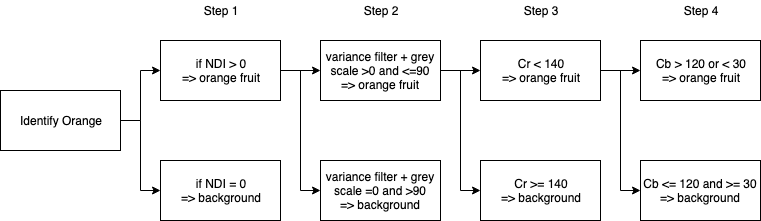
\includegraphics[width=0.5\textwidth]{algo_stages}}
\caption{Outline of the proccess of the stages of the algorithm}
\label{fig}
\end{figure}

\subsection{Stages}

\subsubsection{Step 1}
The first step in this algorithm is to produce a normalised index between the red and green channels. The index is calculated such that $NDI = (g - r) / (g + r)$ for each pixel in both channels. The values are then thresholded where $NDI > 0$. This step helps provide emphasis on regions with higher redness levels, and less emphasis on foliage.

\subsubsection{Step 2}
In Payne’s algorithm, a $3x3$ variance filter is used for each colour channel, then combined and converted to grayscale, and finally thresholded to meet a desired property. This process provided to be insufficient for oranges, and instead a $3x3$ adaptive mean threshold filter was used. This new filter was able to remove excess foliage from the image, as well as remove areas that are irrelevant to the oranges, such as the sky.

\subsubsection{Step 3}
The image is then converted into YCbCr colour space, and Cr and Cb channels extracted to threshold from. The Cr channel measures the red difference within the image, so any component which favours a medium to high red level will work. As such, the threshold value of $pixelvalue >= 140$ is used, as this was seen to be the average minimum Cr value found across multiple images containing oranges.

\subsubsection{Step 4}

The Cb channel is used to determine the blue difference within the image. This means that a lower to medium value is acceptable for oranges, as this would produce an orange colour when combined with the Cr channel. As such, a threshold condition of $30 <= pixelvalue <= 120$ is used.

\subsubsection{Step 5}

With all of the masks created, they are then combined together to form a final mask using equation \ref{eq:mask}. This mask will select only orange components of the image.

\begin{equation} \label{eq:mask}
pixel_{final}=pixel_{NDI} \land pixel_{mean} \land pixel_{Cr} \land pixel_{Cb} 
\end{equation}

\subsubsection{Step 6}
The final step is to count the crop yield on the tree. The process is to first apply a Gaussian blur to the image and perform a Hough transform to detect circles. These circles are then analyzed to determine how much of the region contains the selected pixel value, and is of reasonable size. Once each circle is checked, the final result will be an image with orange regions are circled.


\subsection{Circle Filtering}

Once the mask is generated after step 5, that mask will be used to count the number of circles, each circle representing an orange fruit. Pseudo code for this is shown below in Algorithms \ref{circleCountAlg}, \ref{overlapComp}, and \ref{OrangeCountAlg}. The first step in the process is to apply a Gaussian blur to the mask to soften the edges for the edge detection algorithm.  Since the Hough transformation will generate more circles then there actually are oranges, we filtered the number of circles down based on calculating a rolling average of the radius, how many pixels are within the circle, how much of the detected circle is within the frame and how much overlap there is. This is shown below in algorithm \ref{circleCountAlg} and discussed below.


\begin{algorithm} 
    \SetKwInOut{Input}{Input}
    \SetKwInOut{Output}{Output}

    \underline{function CountCircles} $(img)$\;
    \Input{Binarized image of the oranges $img$}
    \Output{$NumOranges$}
    
    img = medianBlur(img, 3)
    circles = HoughCircles(img, 2.5, 150, 100, 100, 0, 3000)
    
    found = fillZero(img.size)
    averageR = 0
    
    \For{circle $\in$ circles}{
     ratio = countWhitePixels(img, circle) \label{alg:CountCircle:line_1}
     
     notTakenRatio = countNotTaken(found, circle)  \label{alg:CountCircle:line_2}
     
    \uIf{$circle.radius > img.size/4 \lor ratio <  20$}
      {
        continue
      }
      
      /* make sure that the radius does not differ too much */
      
      \If{$(averageR = 0) \lor (averageR\cdot0.5 \leq circle.radius \leq averageR\cdot1.5$}
      {
      	/* very confident this is an orange*/
	
          \If{$ratio \geq 50$}	
          {
          	averageR = (averageR +  circle.radius) / 2
	
		markFound(found, circle)
		
		markCircle(img, circle, color.GREEN)
	  }
	  \ElseIf{$ratio \geq 30$}{
	  
	  	 \uIf{$averageR\cdot0.8 \leq circle.radius \leq averageR\cdot1.2$}	
          	{
			markCircle(img, circle, color.ORANGE)
	 	 }
	  	\uElseIf{$ circle.radius \leq averageR\cdot1.4$}{
			markCircle(img, circle, color.PURPLE)
	  	}
		\uElse{
			markCircle(img, circle, color.RED)
		}
	  }
	  \Else{
	  	/* not filled enough, but close size*/
		
		\uIf{$averageR\cdot0.8 \leq circle.radius \leq averageR\cdot1.2$} {
			markCircle(img, circle, color.MAROON)
		}
	  }
      }
    }
    \caption{Orange counting algorithms} \label{circleCountAlg}
\end{algorithm}


The values that were selected for the Hough transform were chosen as; $dp = 2.5$, $minDist = 150px$, $thresholds = 100$, $minimum radius = 0$, and  $maximum radius = 3000$. The $dp$ is an inverse ratio used in the accumulator which is used to detect circles, we chose this value based on running the algorithm with multiple images and this yielded the best result. The value of 150px was chosen to be the minimum distance because most of the images were large enough that this value did not cause a significant number of the oranges to be missed. This is discussed in more detail in section \ref{sec:limitations}. The 2 Hough transform parameters that are used for Canny Edge detection were set to 100, an arbetrary value between 0 and 255, since the base image that was being used had been previously binarized to contain only values of 0 and 255 (not including the Gaussian blur on the edges). \cite{yadav_approach_2014}.


On line \ref{alg:CountCircle:line_1} in algorithm \ref{circleCountAlg}, the percentage of pixels in the image that have been identified as part of the orange is taken to the number of pixels within the circle that are not part of the orange. Details of this are shown in algorithm \ref{OrangeCountAlg}. The White count algorithm takes into account part of the detected circle that is outside of the frame of the image, if less than 40\% if the circle is outside the frame then that portion that is outside is assumed to be filled, if more then 40\% is outside then it is assumed to not be filled. 


On line \ref{alg:CountCircle:line_2} of algorithm \ref{circleCountAlg}, the percentage of pixels that are not already taken is counted as part of another orange. This reduces the number of overlapping circles that are detected. This can be seen in figure \ref{overlapComp} where the image on the right does not filter the circles by how much they overlap and the one one on the right does. Details of this are shown in algorithm \ref{CheckOverlapAlg}


\begin{figure}[H]
  \begin{subfigure}{.49\linewidth}
 	 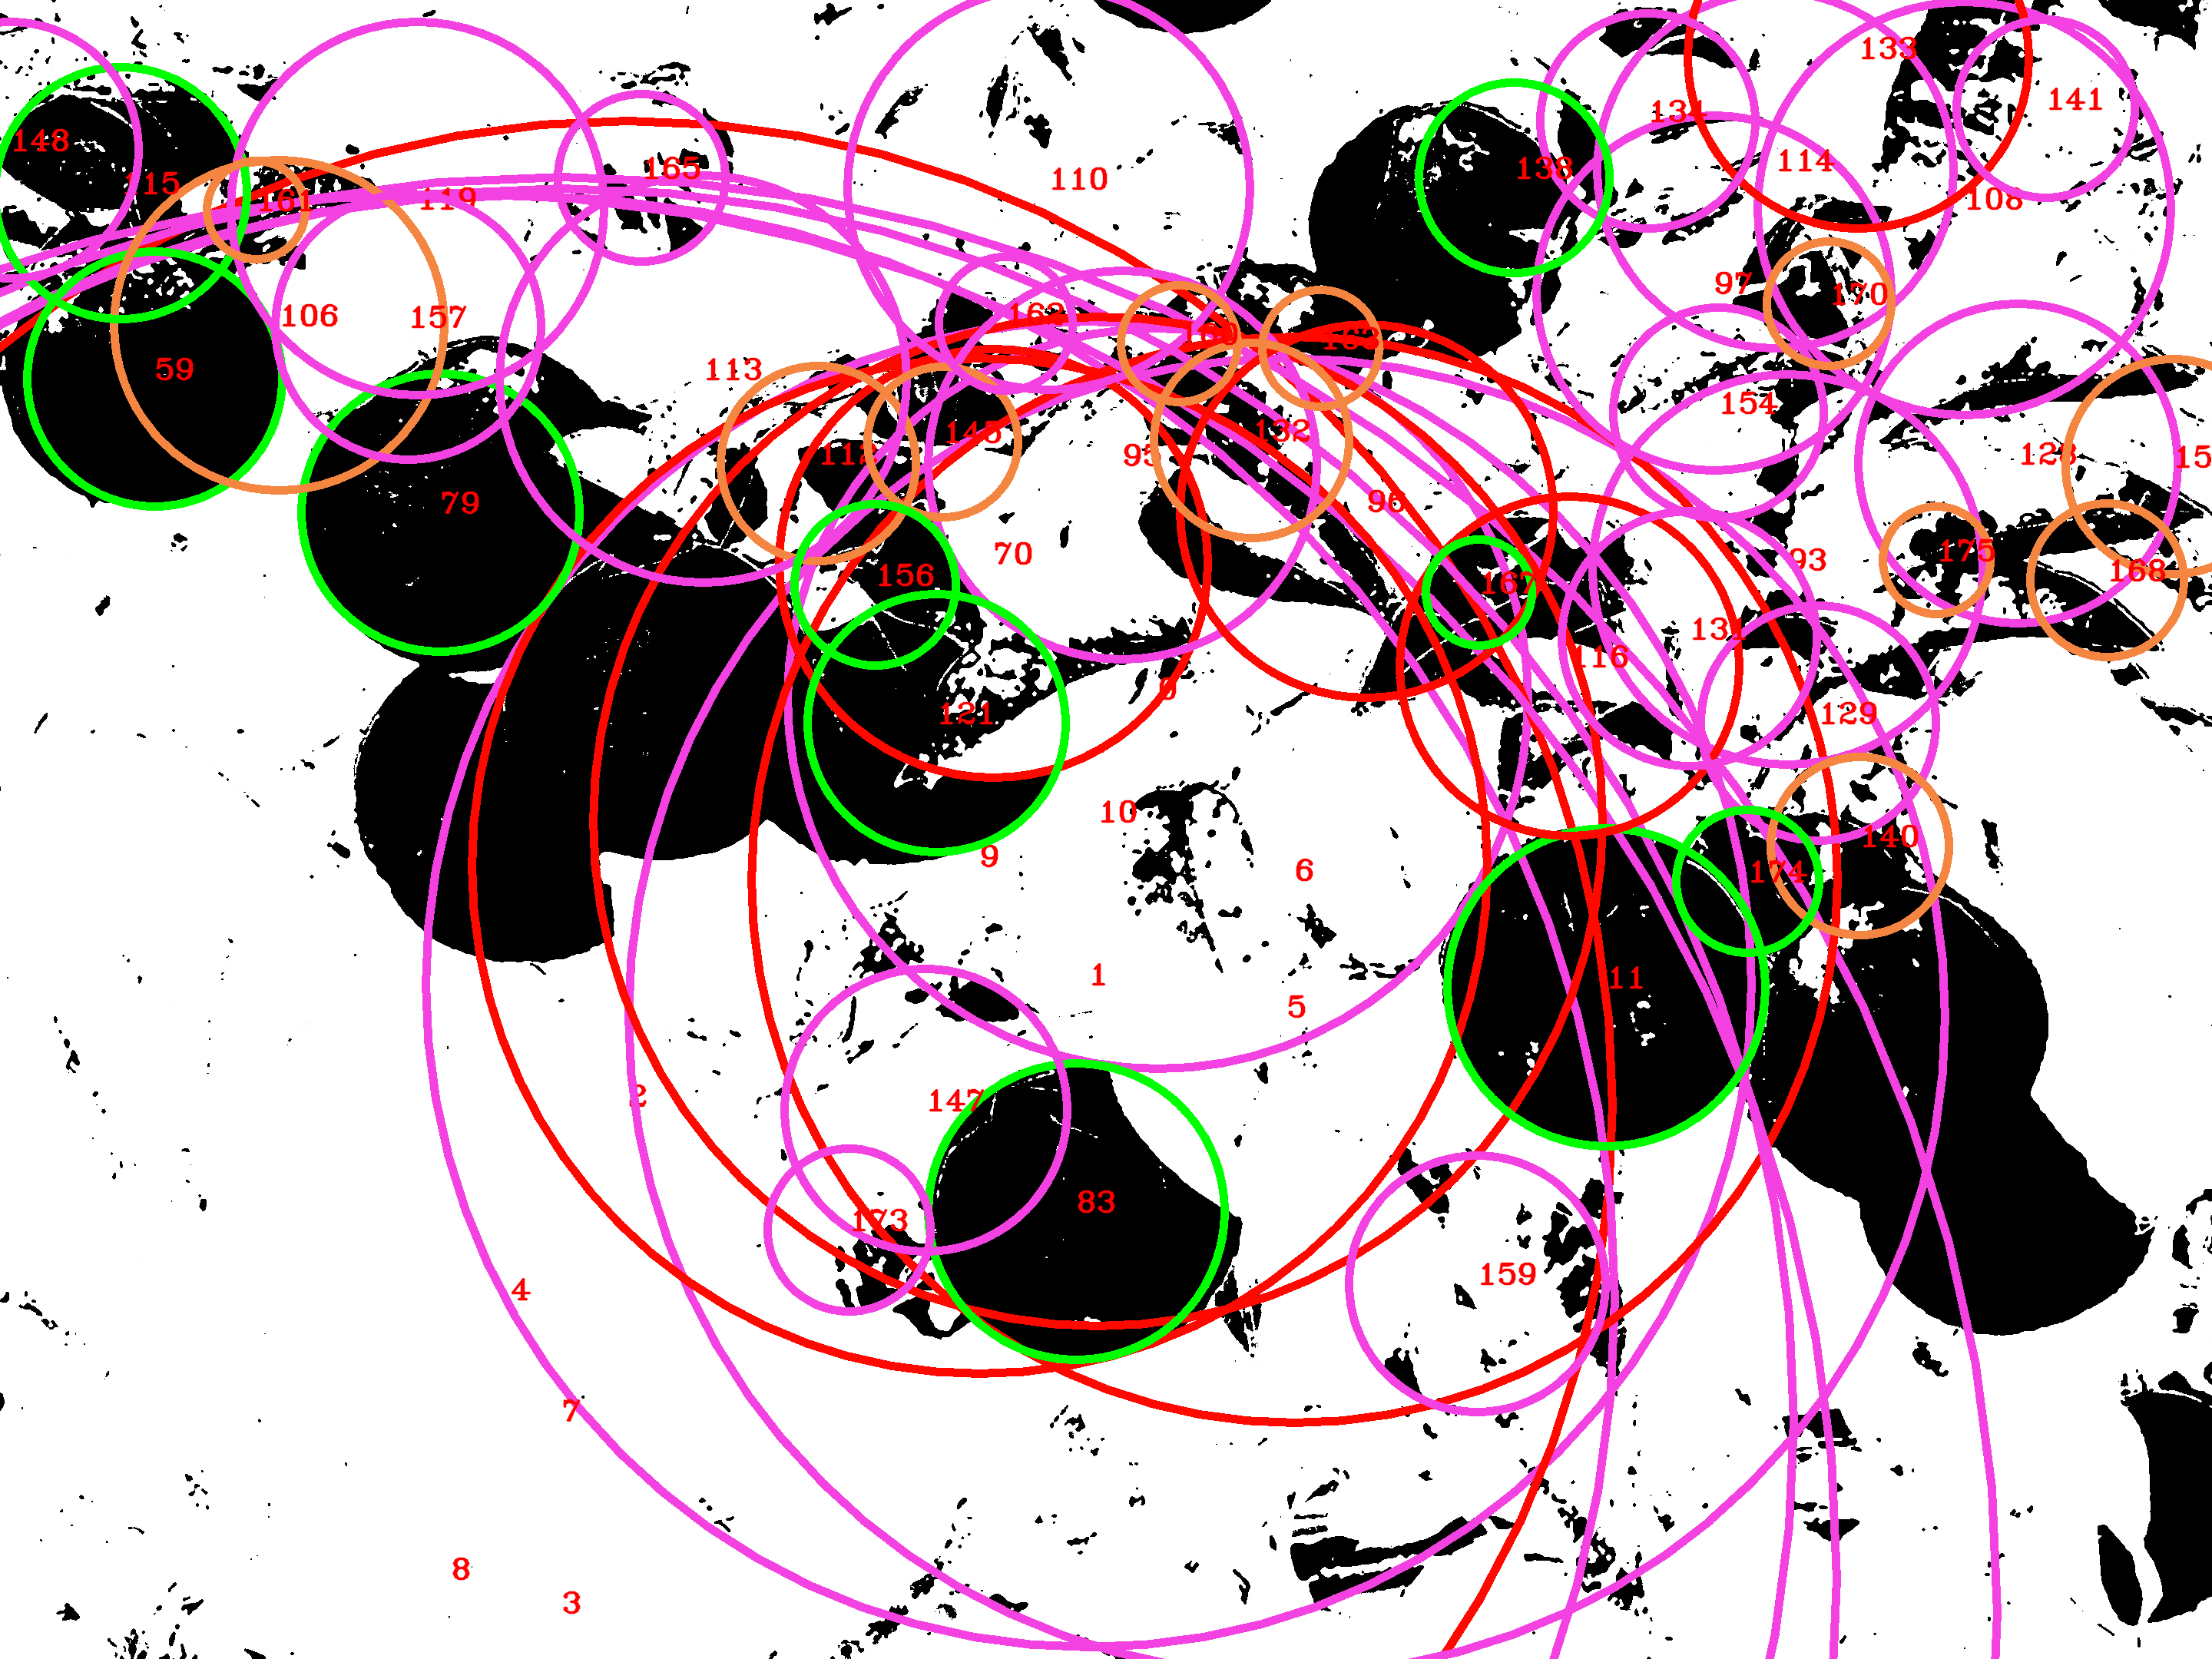
\includegraphics[width=\linewidth]{citrus2_circles.png}\hfill
	 \caption{Filtered out overlapping circles}
  \end{subfigure}
  \begin{subfigure}{.49\linewidth}
  	\includegraphics[width=\linewidth]{citrus2_circles_withoverlapfilter.png}
   	\caption{Oranges with overlapping circles}
  \end{subfigure}
  \caption{An example image going through each step to detect the oranges within the image, (Note: only the green, confident detections are shown for the sake of simplicity)} \label{overlapComp}
\end{figure}


The circle counting algorithm produces various different circles for the oranges as can be seen in fig. \ref{fig:citrus_results}. Each circle colour represents how confident that the algorithm is that that circle is an orange. They are listed below in decreasing order of confidence.

\begin{itemize}
\item Green - over 50\% filled, within 50\% of the other green circles
\item Orange - over 30\% filled, within 20\% of the green circle sizes
\item Red - over 30\% filled, smaller than 40\% larger than the green circle sizes
\item Maroon - under 30\% filled,  within 20\% of the green circle sizes
\item Purple - over 30\% filled, larger  than 40\% bigger than the green circle sizes
\end{itemize}


\section{Results}

The algorithm was tested against a set of 8 images, each with varying brightness and foliage levels. Among all of the images, there is approximately a 73\% success rate for detecting the oranges with high confidence. There are also results for each image where the algorithm is only moderately confident in the result, with each image having around 1-2. In each resulting image, oranges with high confidence are highlighted in a green circle, and those with moderate confidence are circled in orange. For example, the image "citrus\_1" in fig. \ref{fig:citrus_results_1} detects 24 out of the 32 possible oranges within the image, missing those that are mostly covered in foliage. Same thing can be seen for "citrus\_3" in fig. \ref{fig:citrus_results_3} , with 10 oranges detected out of the possible 14. It can be seen that the images with high levels of brightness cause the algorithm to become less accurate, with images "citrus\_6"  in fig.\ref{fig:citrus_results_6} and "citrus\_8" in fig. \ref{fig:citrus_results_8}  having approximately 0.1\% accuracy each. Finally, there are cases where an orange is counted twice, which can be seen in the images "circles\_3" in fig. \ref{fig:citrus_results_3} and "circles\_4" in fig. \ref{fig:citrus_results_4} .

\begin{figure}[H]
  \begin{subfigure}{.3\linewidth}
 	 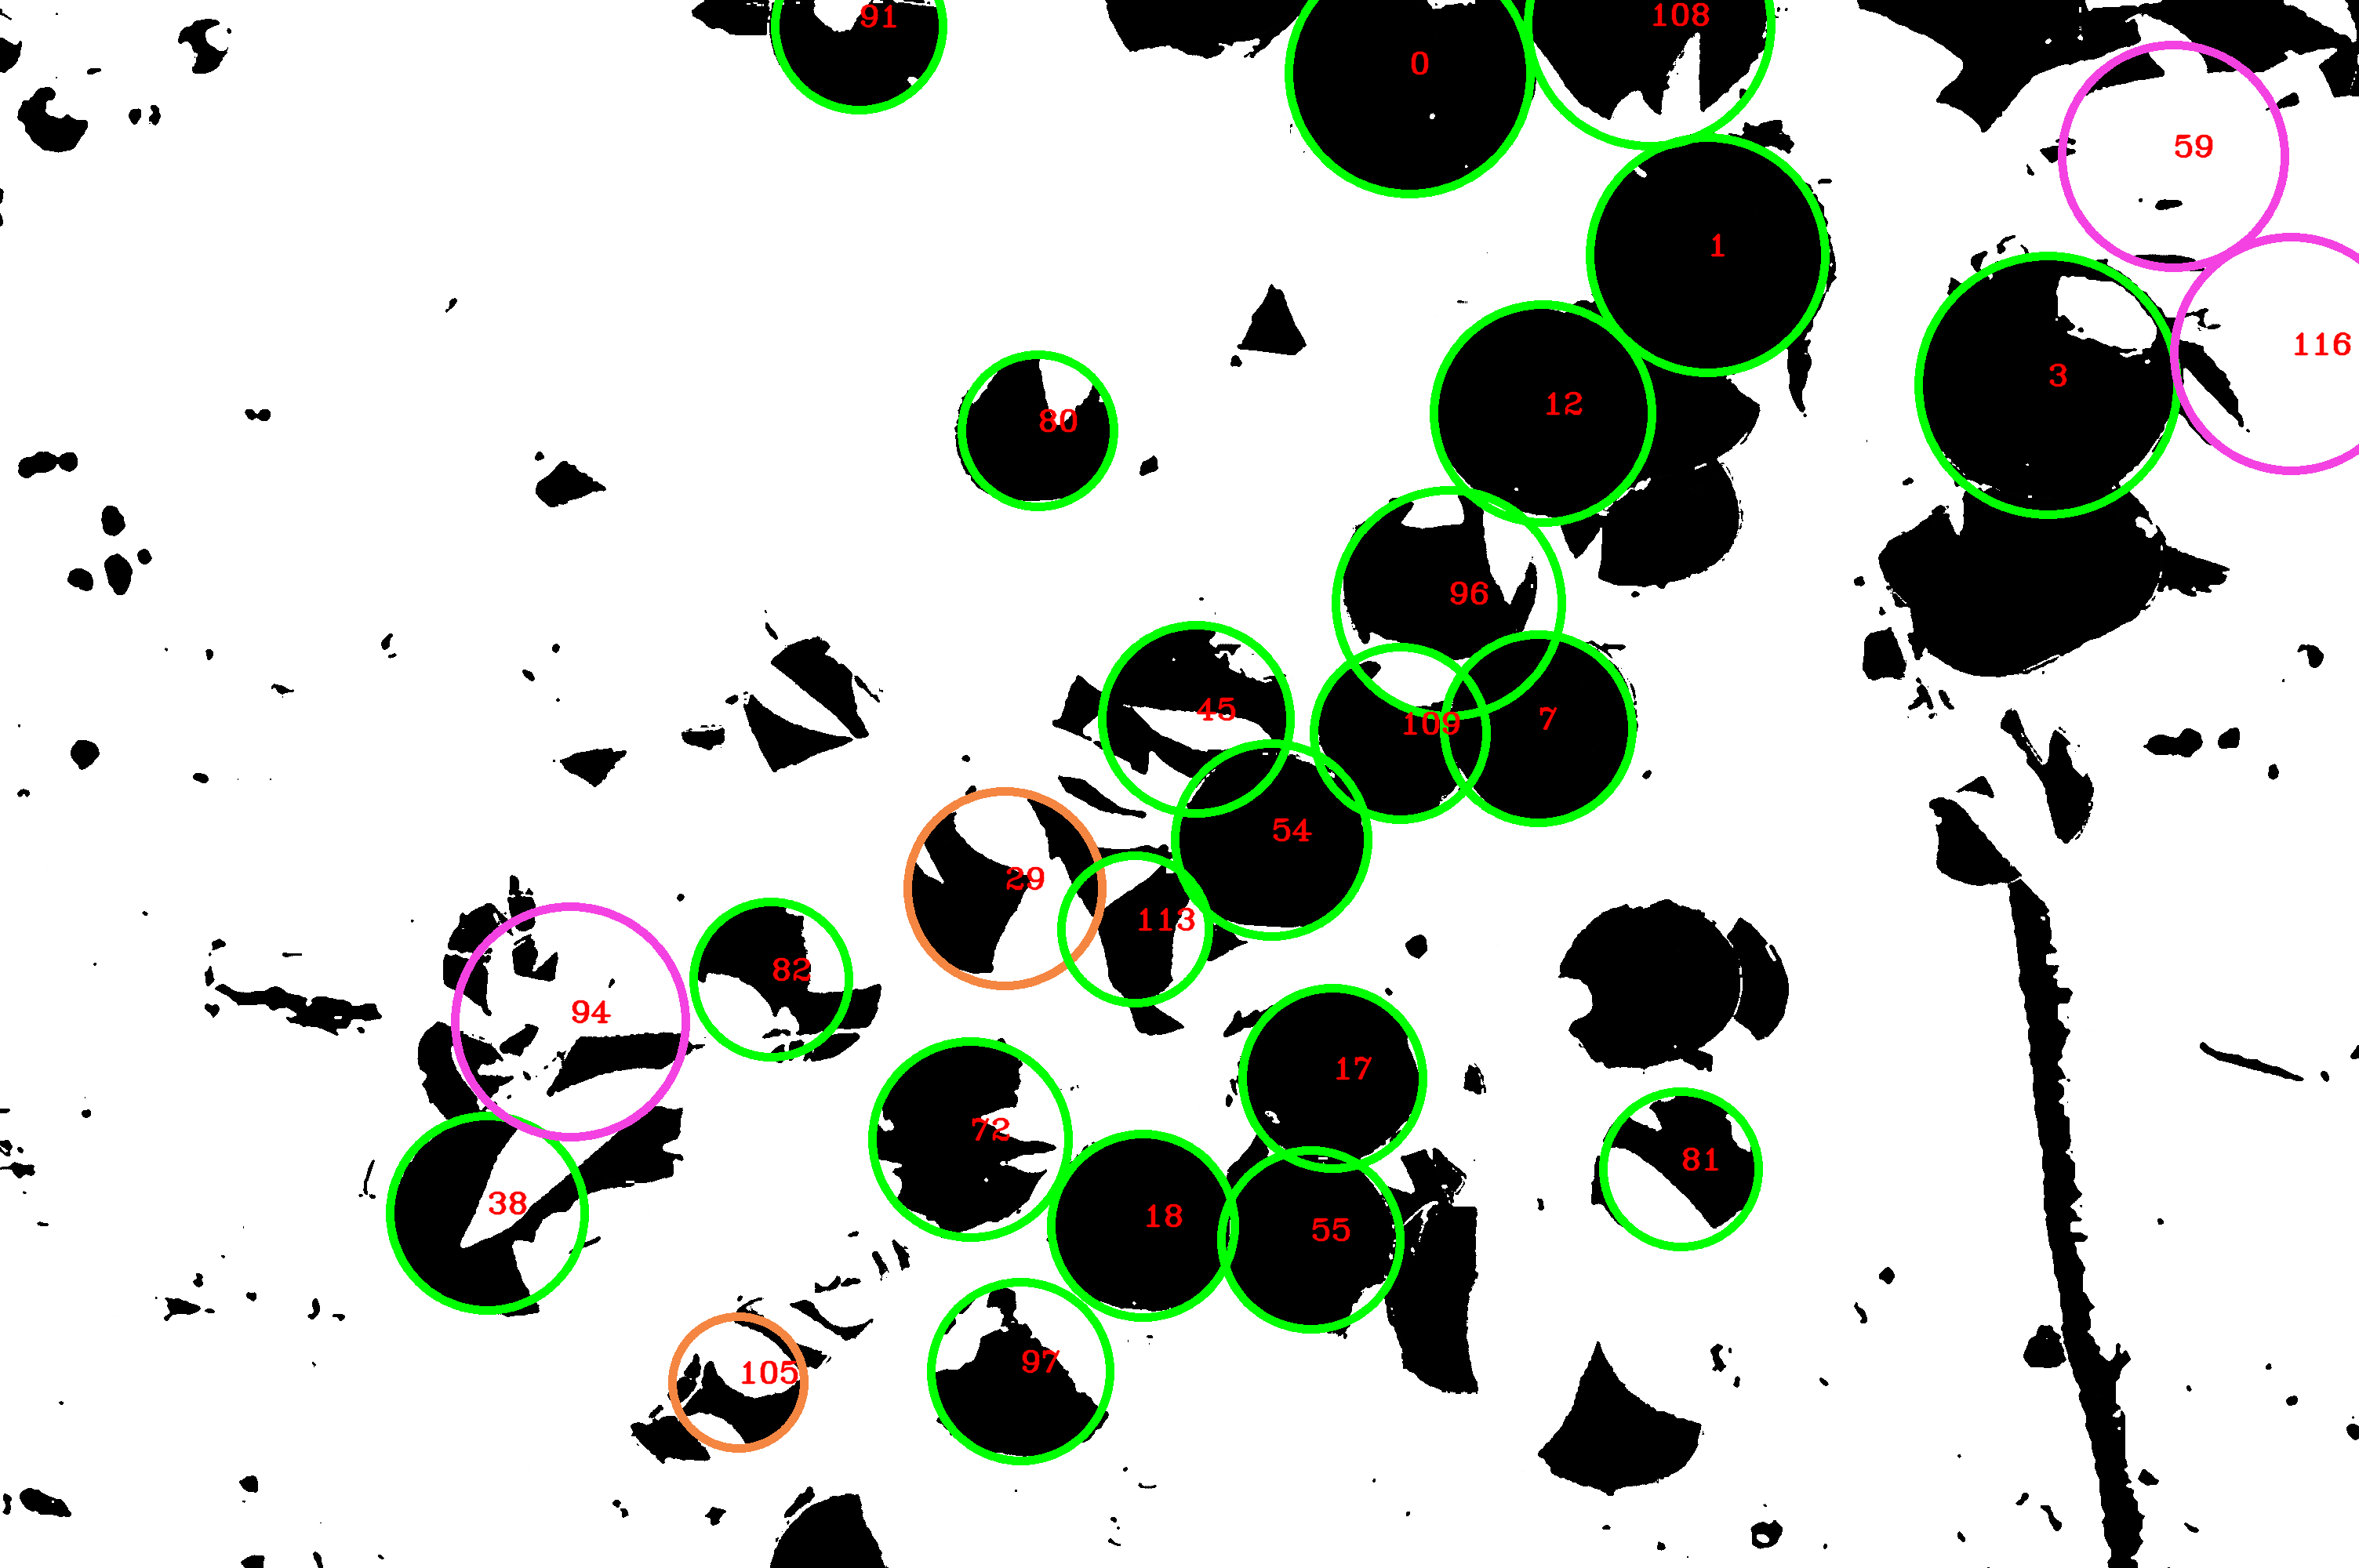
\includegraphics[width=\linewidth]{citrus1/citrus1_circles.png}\hfill
	 \caption{Citrus 1} \label{fig:citrus_results_1}
  \end{subfigure}
   \begin{subfigure}{.3\linewidth}
 	 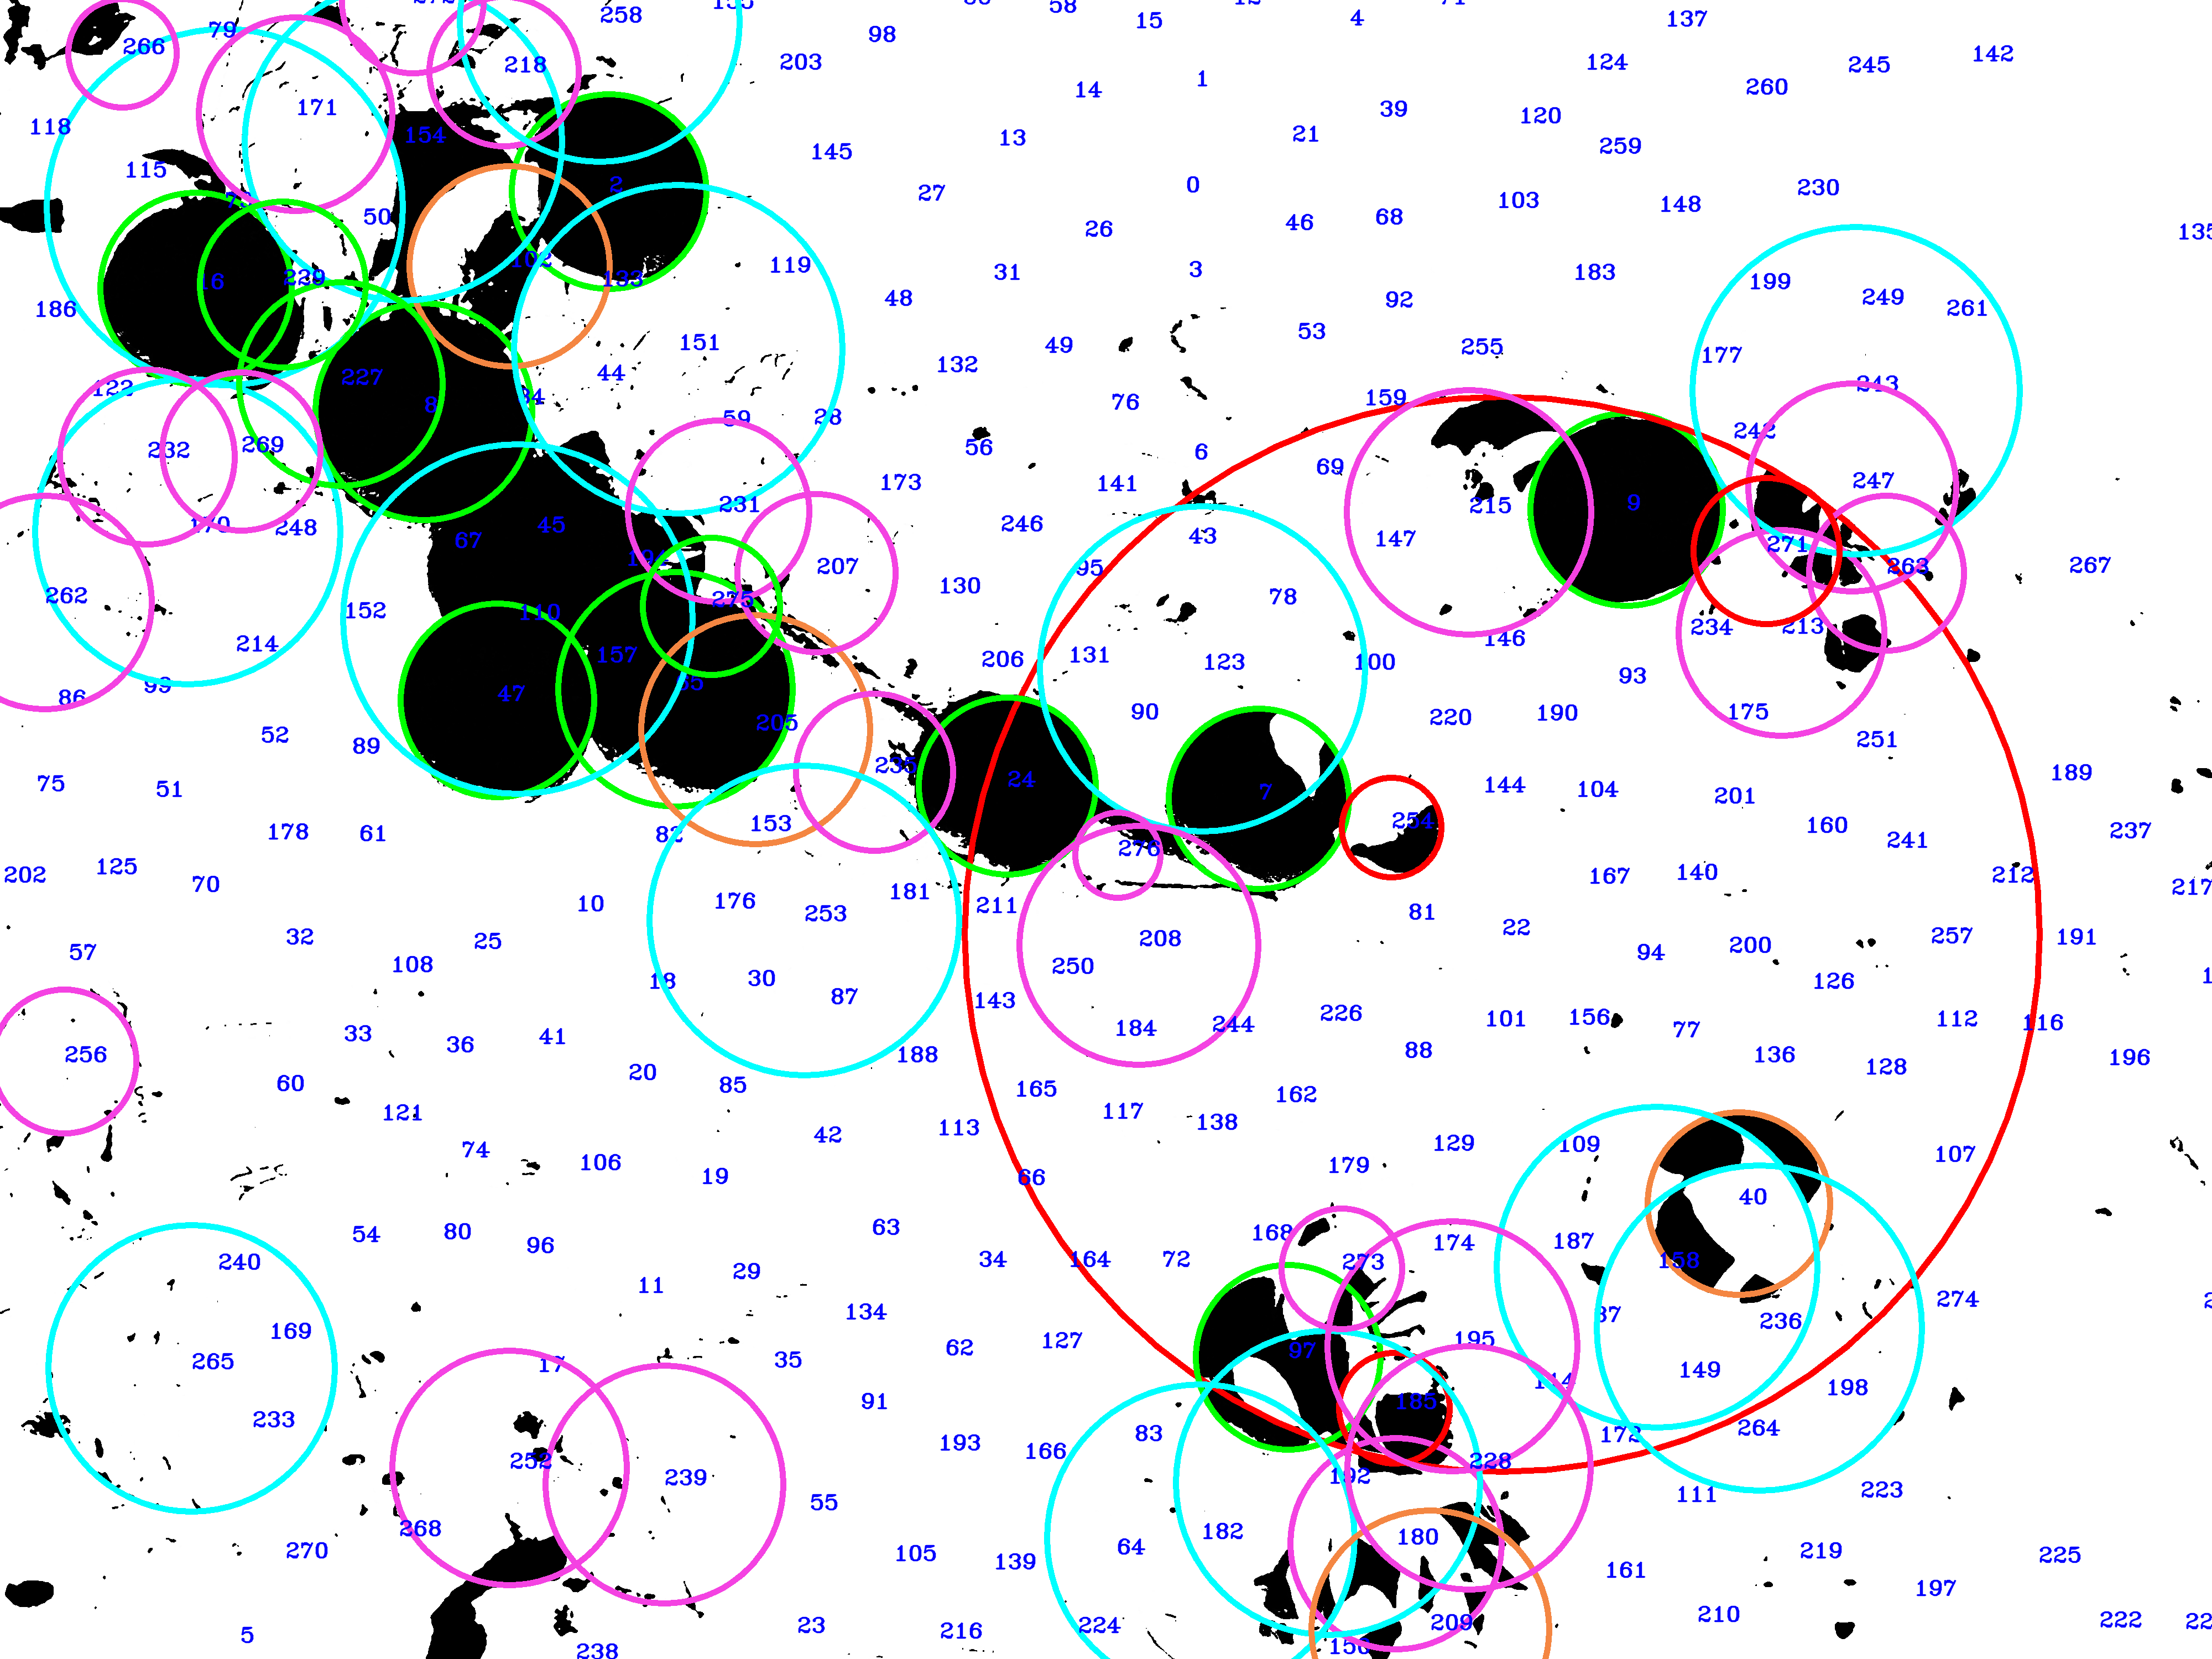
\includegraphics[width=\linewidth]{citrus3_circles.png}\hfill
	 \caption{Citrus 3}  \label{fig:citrus_results_3}
  \end{subfigure}
   \begin{subfigure}{.3\linewidth}
 	 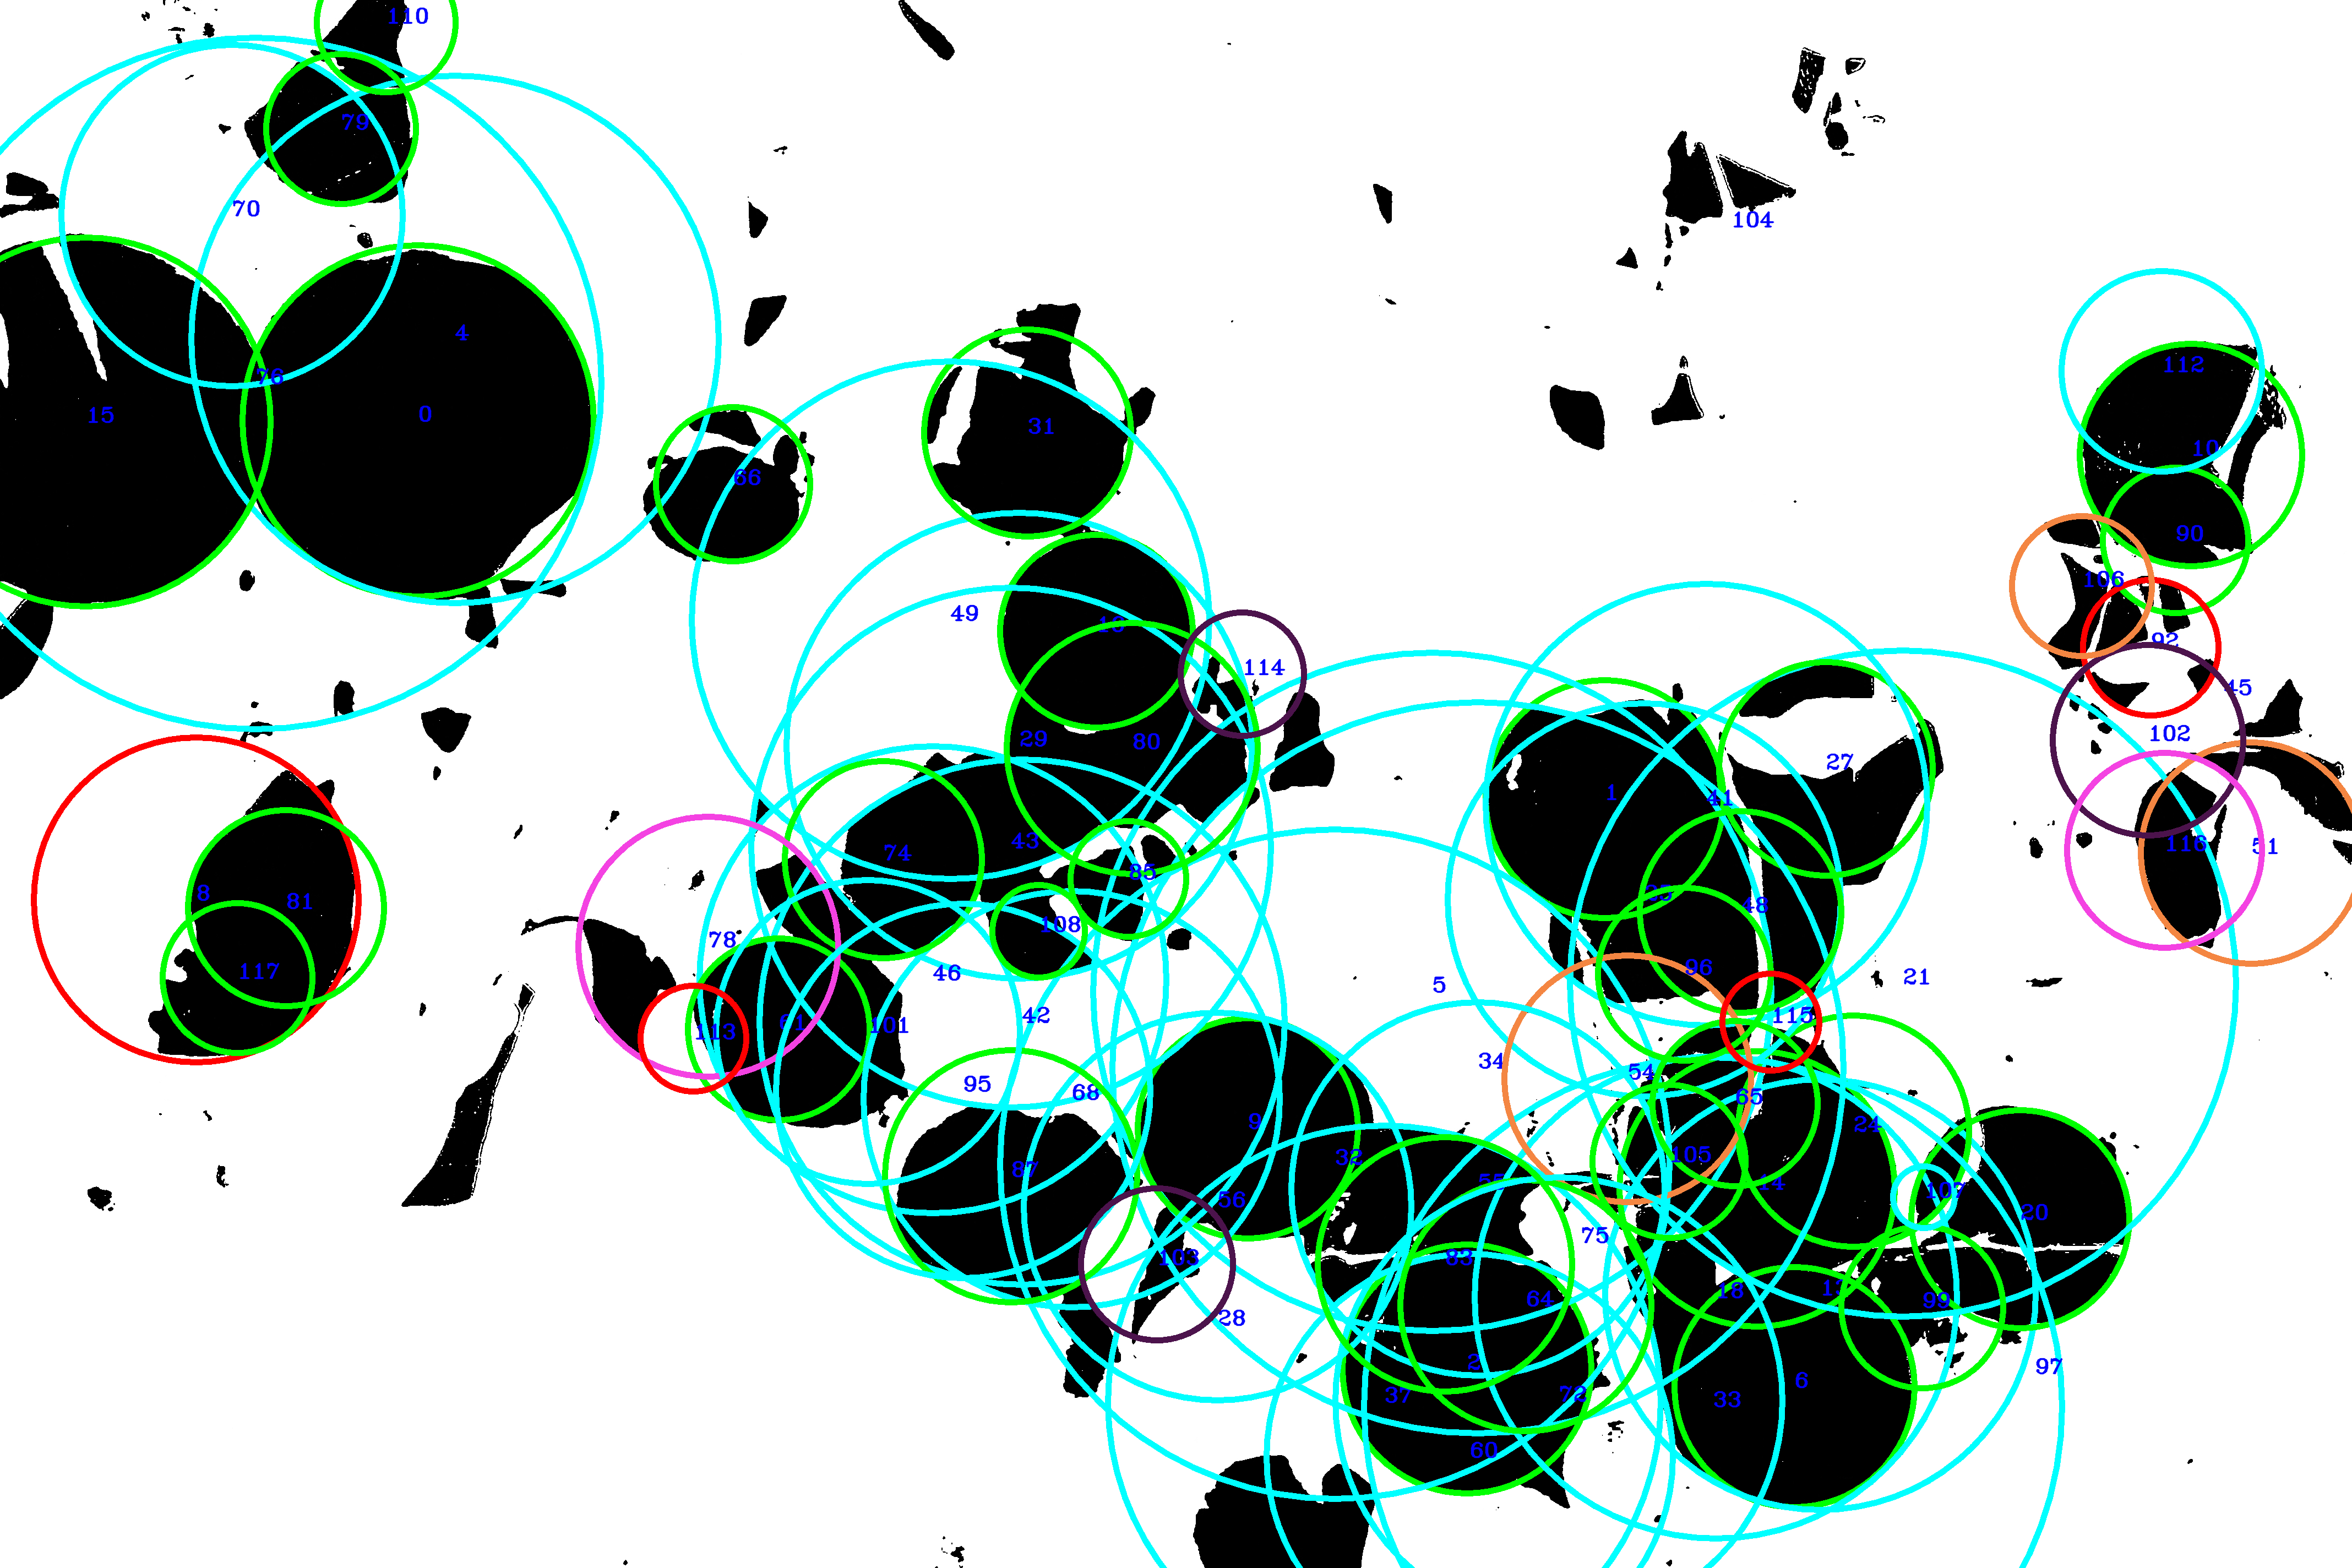
\includegraphics[width=\linewidth]{citrus4_circles.png}
	 \caption{Citrus 4}  \label{fig:citrus_results_4}
  \end{subfigure}\par\medskip
  
    \begin{subfigure}{.3\linewidth}
 	 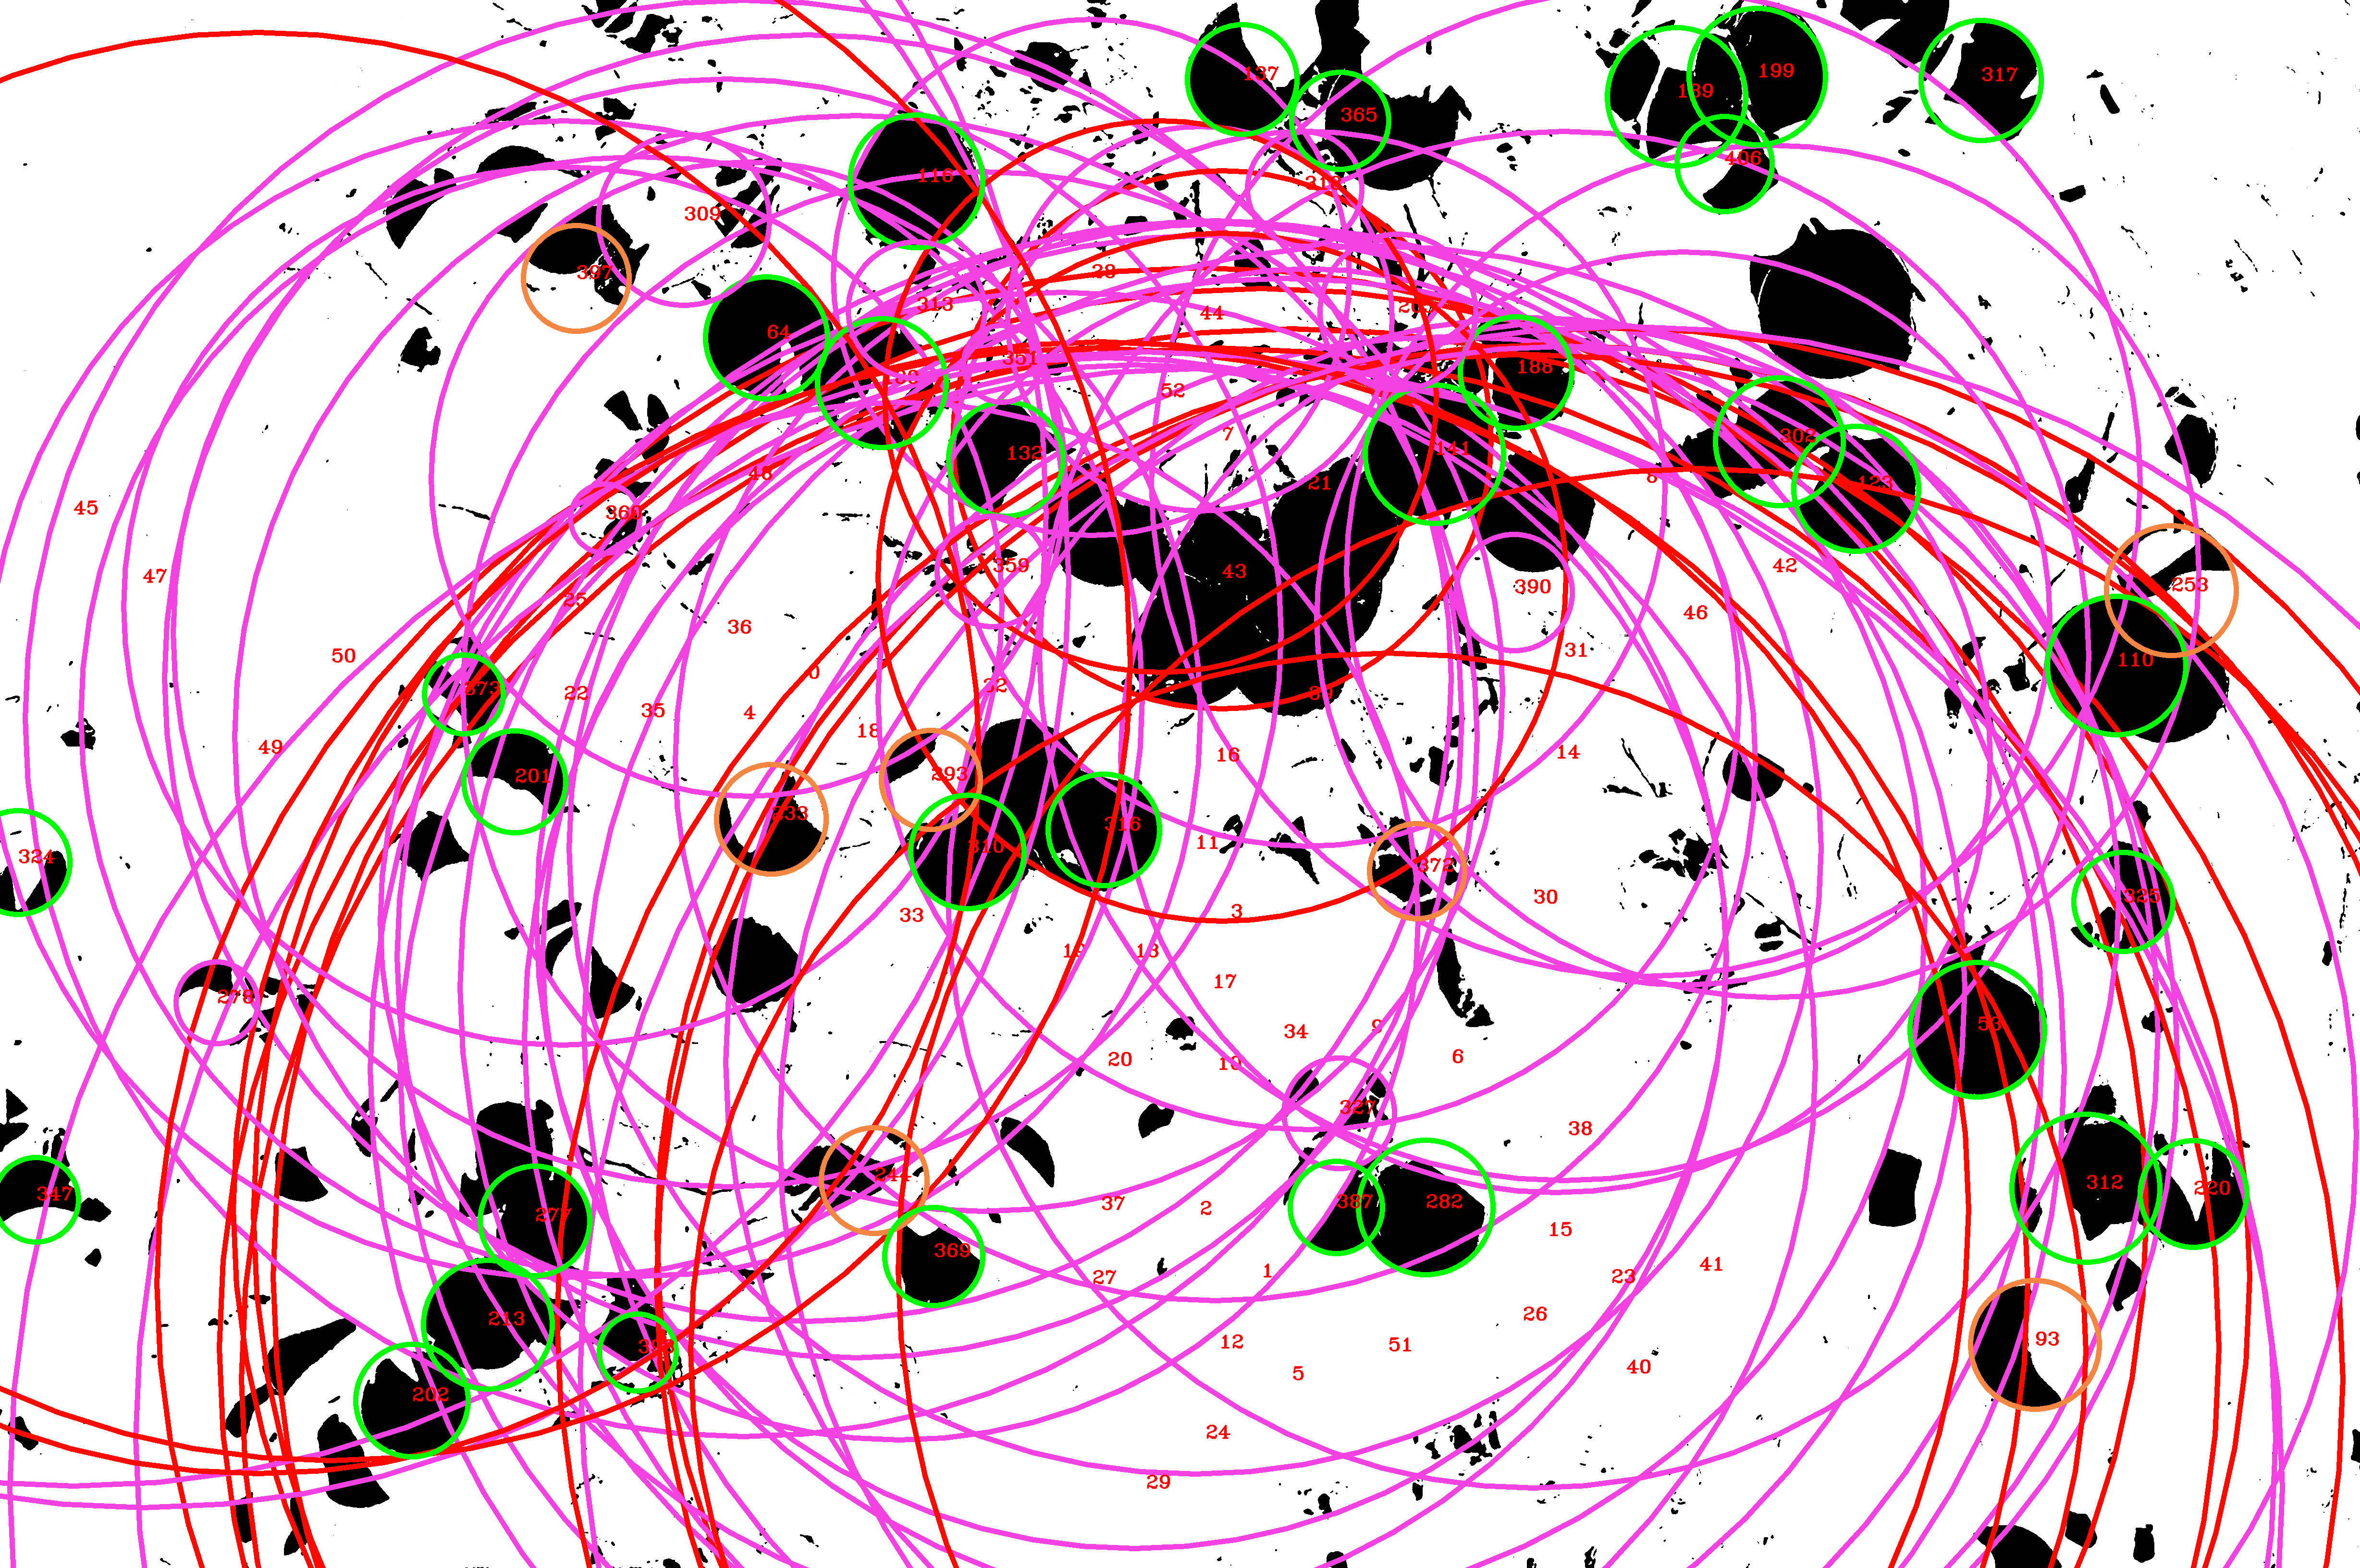
\includegraphics[width=\linewidth]{citrus6_circles.png}\hfill
	 \caption{Citrus 6}  \label{fig:citrus_results_6}
  \end{subfigure}
   \begin{subfigure}{.3\linewidth}
 	 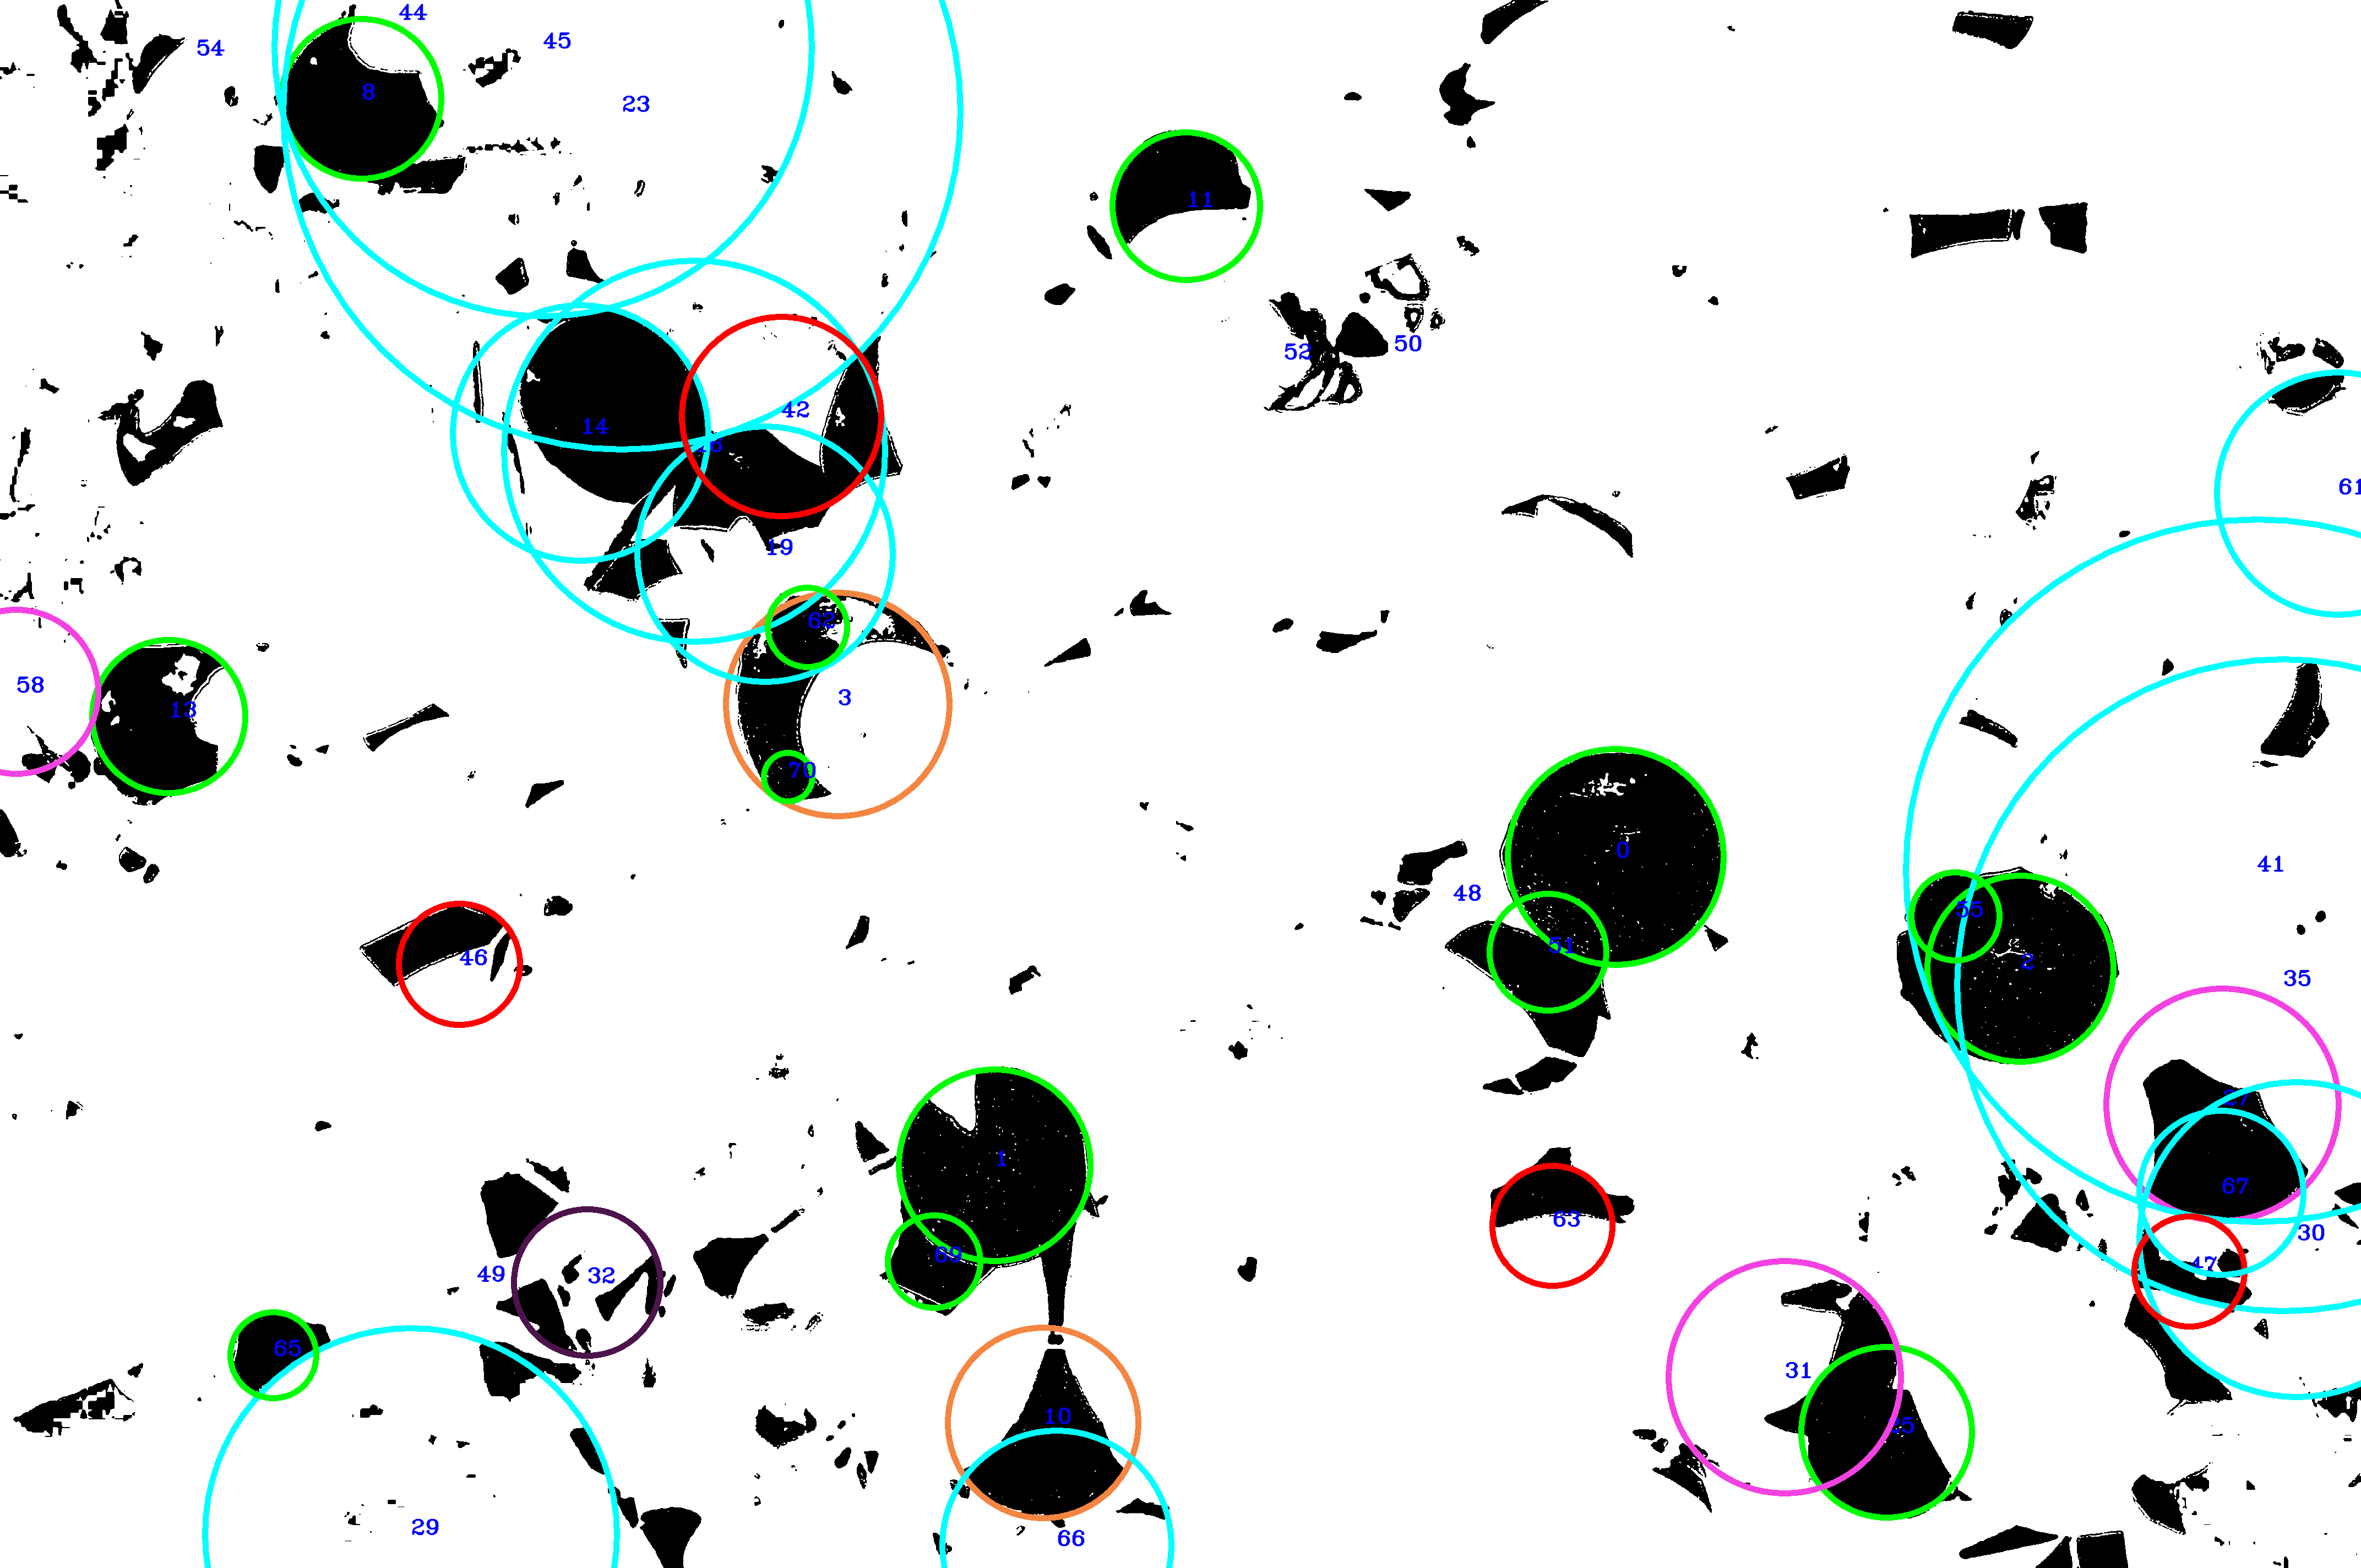
\includegraphics[width=\linewidth]{citrus8_circles.png}
	 \caption{Citrus 8}  \label{fig:citrus_results_8}
  \end{subfigure}
  \caption{The results of the circle counting algorithm} \label{fig:citrus_results}
\end{figure}

In figure 


\begin{figure}[H]
  \begin{subfigure}{.3\linewidth}
 	 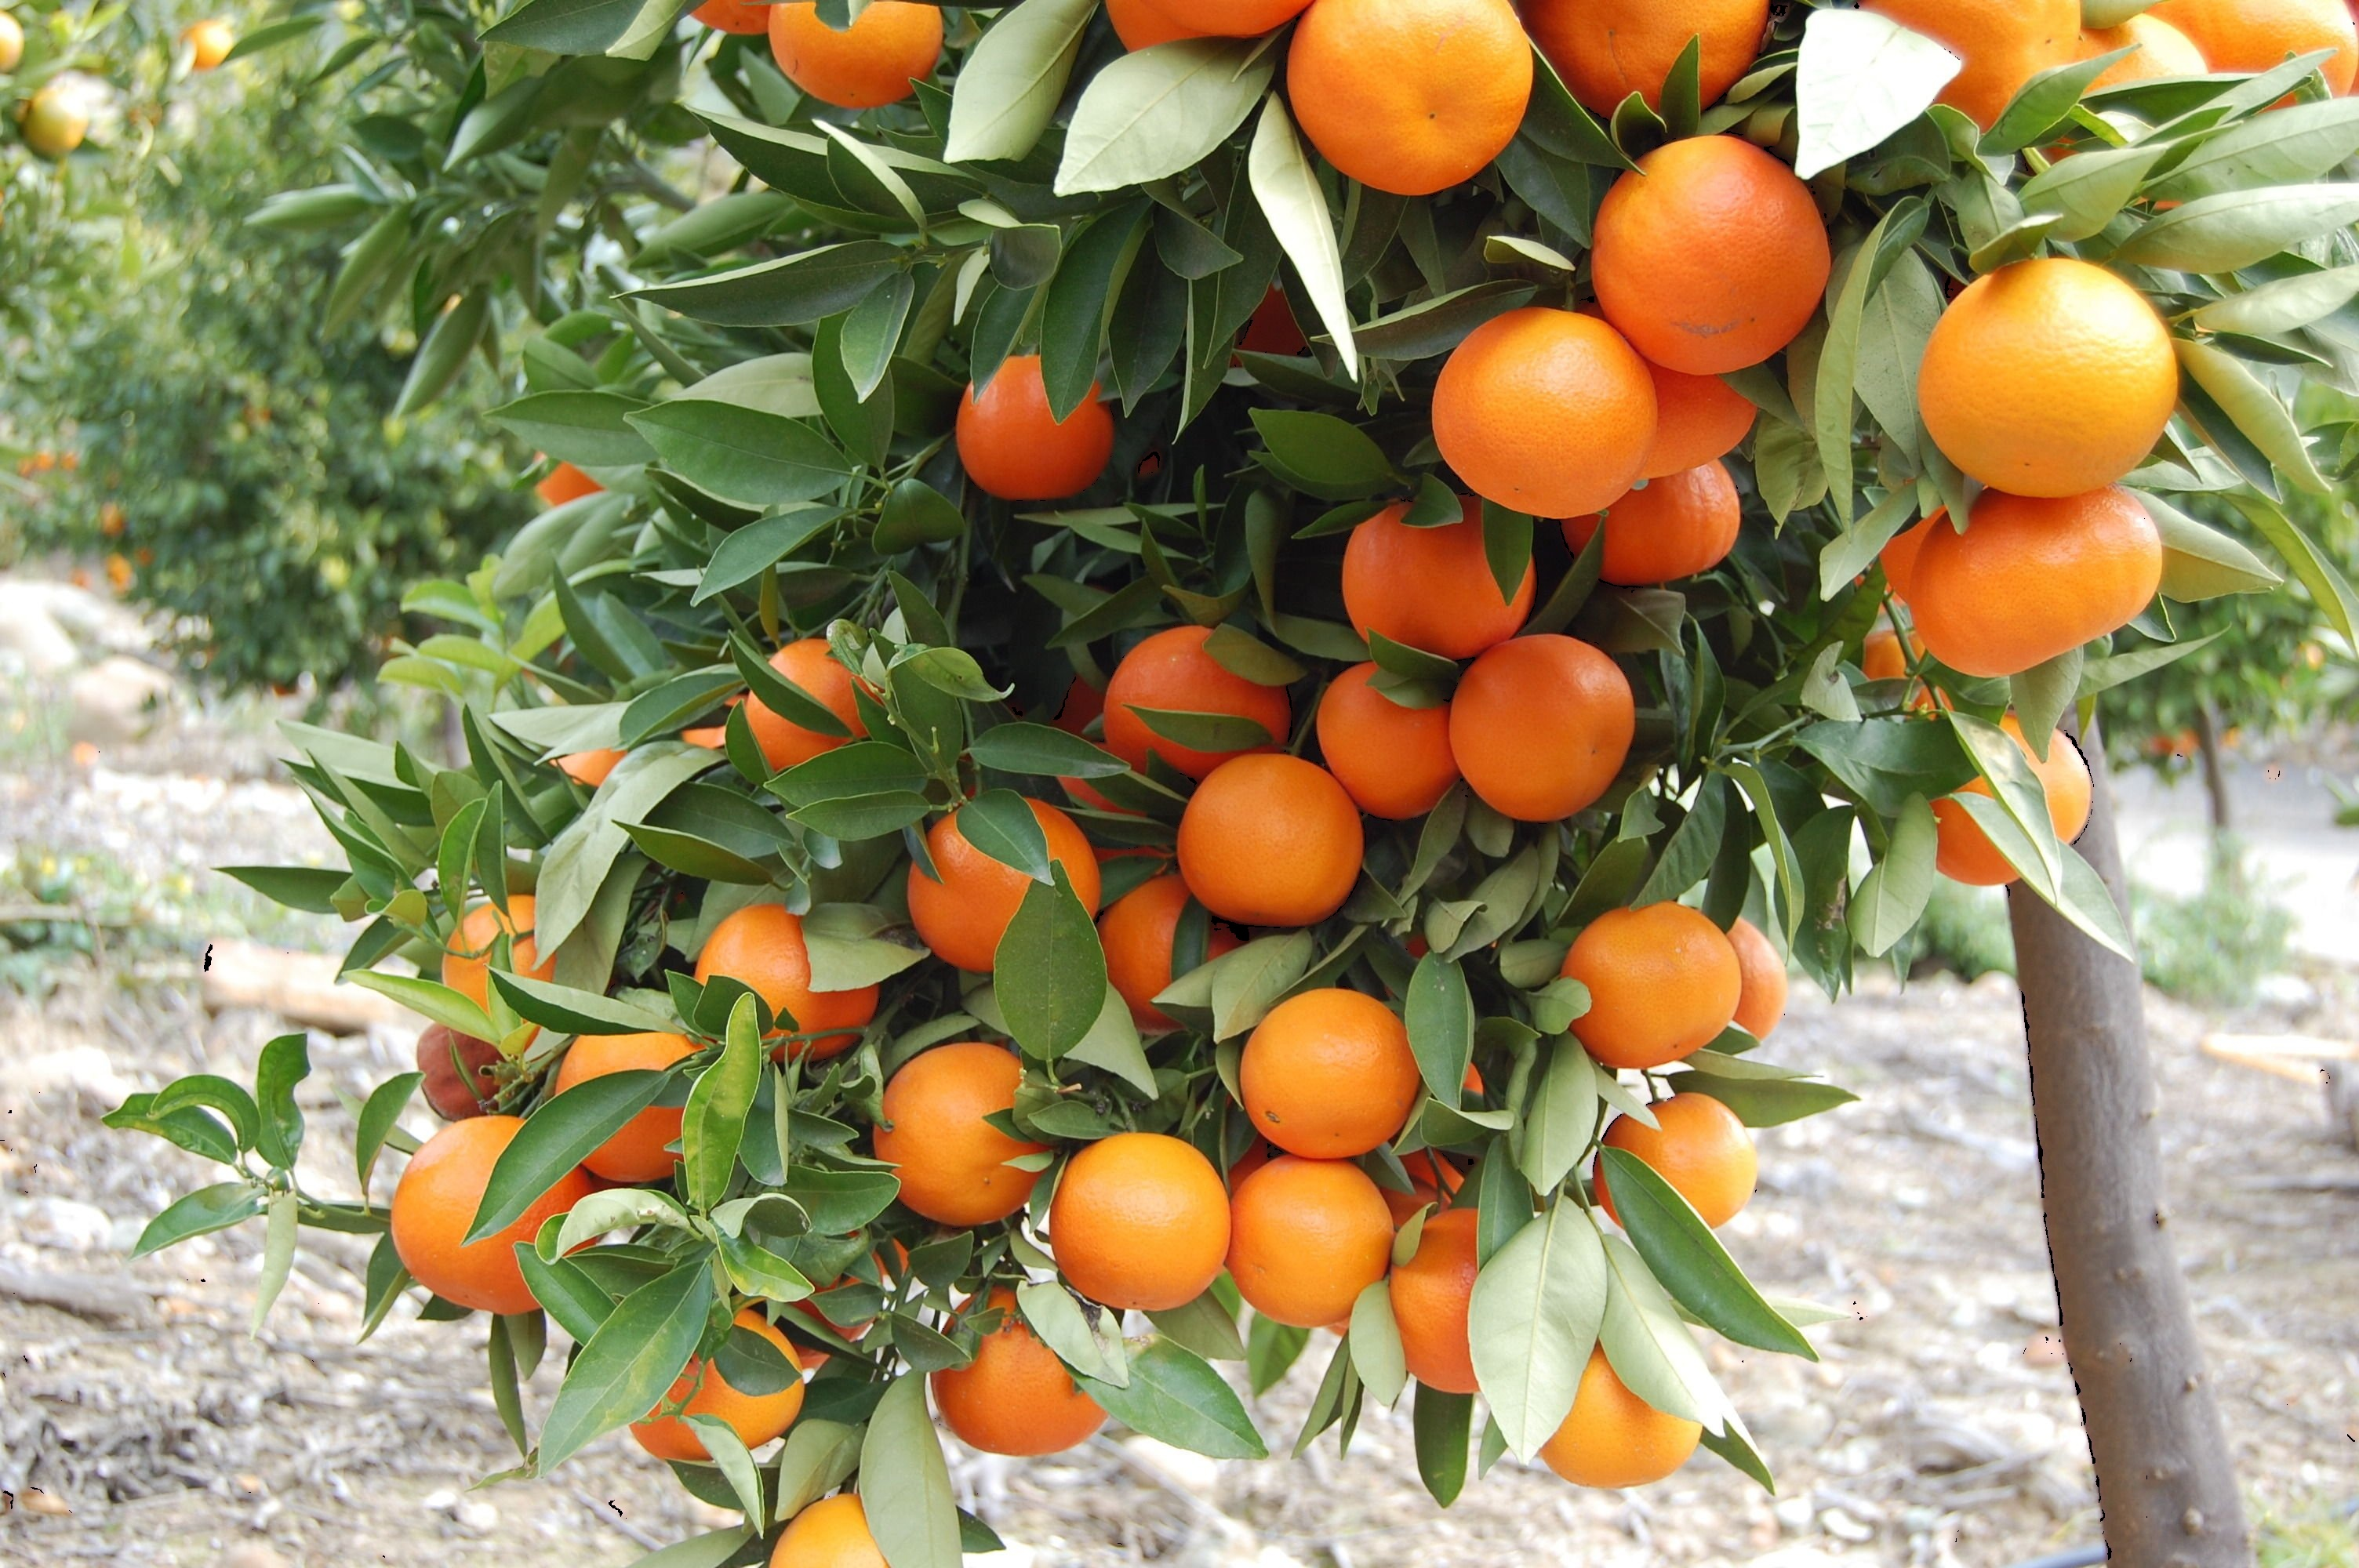
\includegraphics[width=\linewidth]{citrus1/citrus1_orig.jpg}\hfill
	 \caption{Origonal}
  \end{subfigure}
  \begin{subfigure}{.3\linewidth}
  	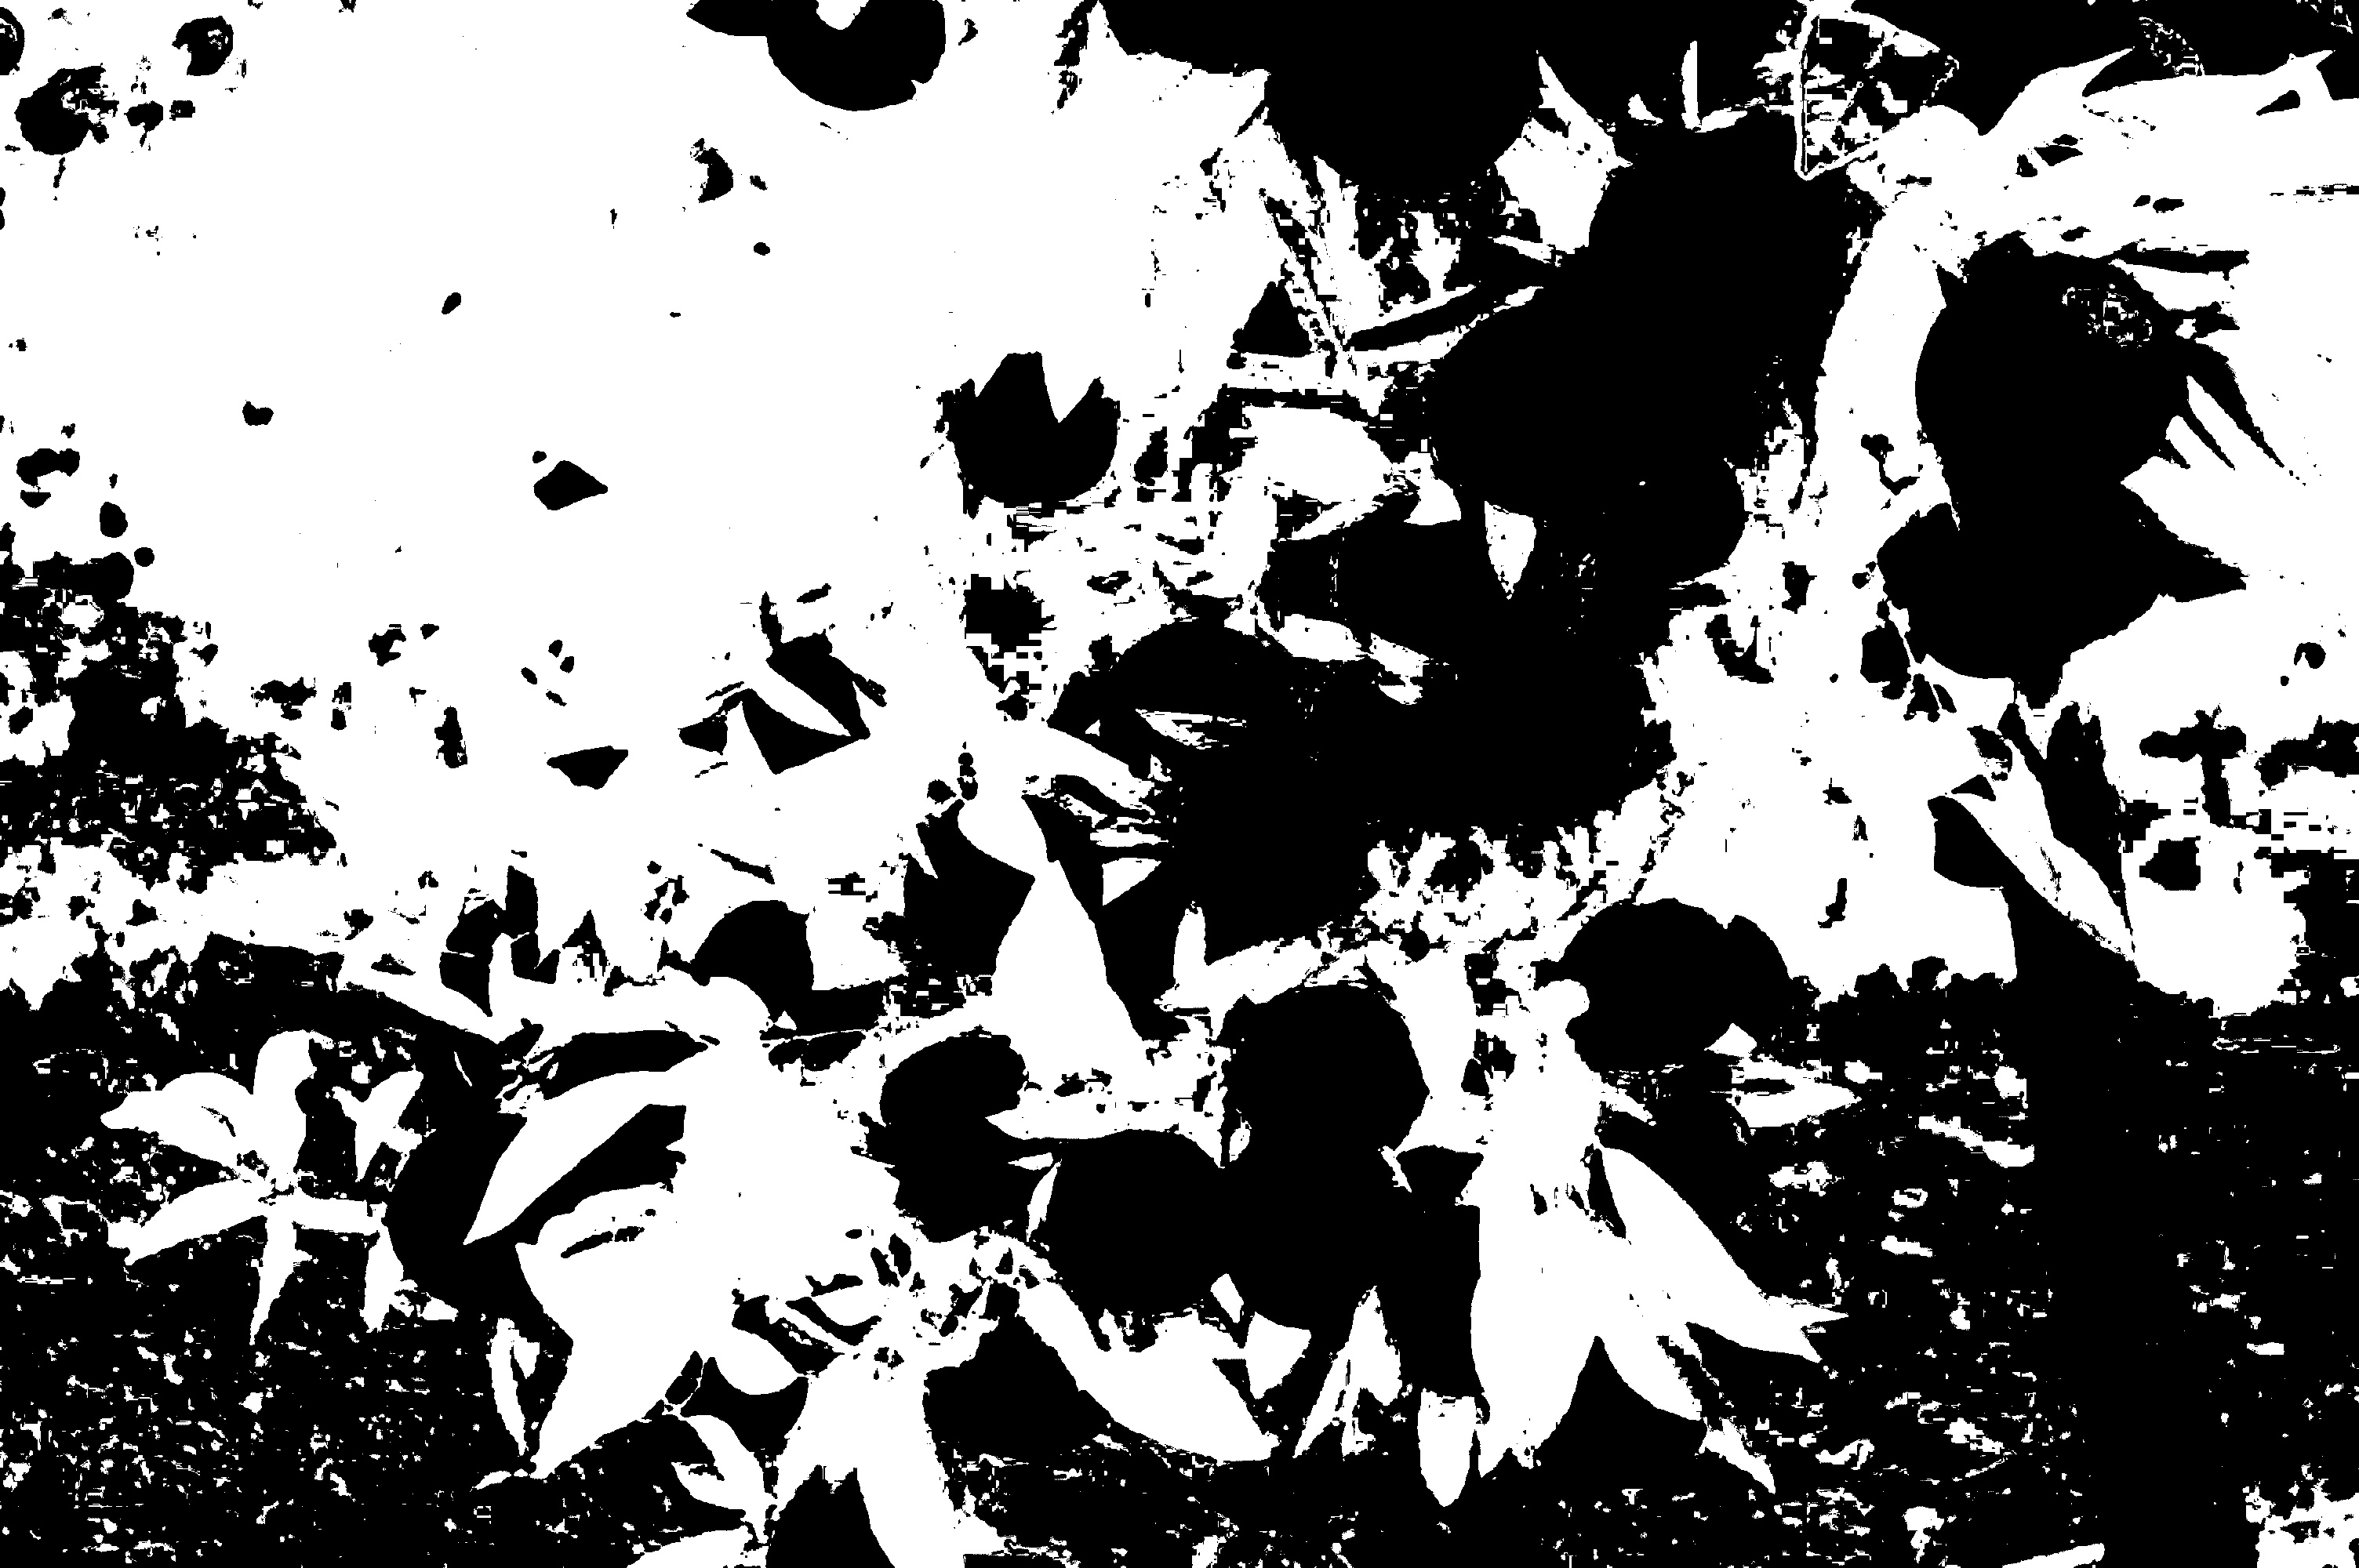
\includegraphics[width=\linewidth]{citrus1/citrus1_NDI.jpg}\hfill
   	\caption{Result of step 1}
  \end{subfigure}
  \begin{subfigure}{.3\linewidth}
  	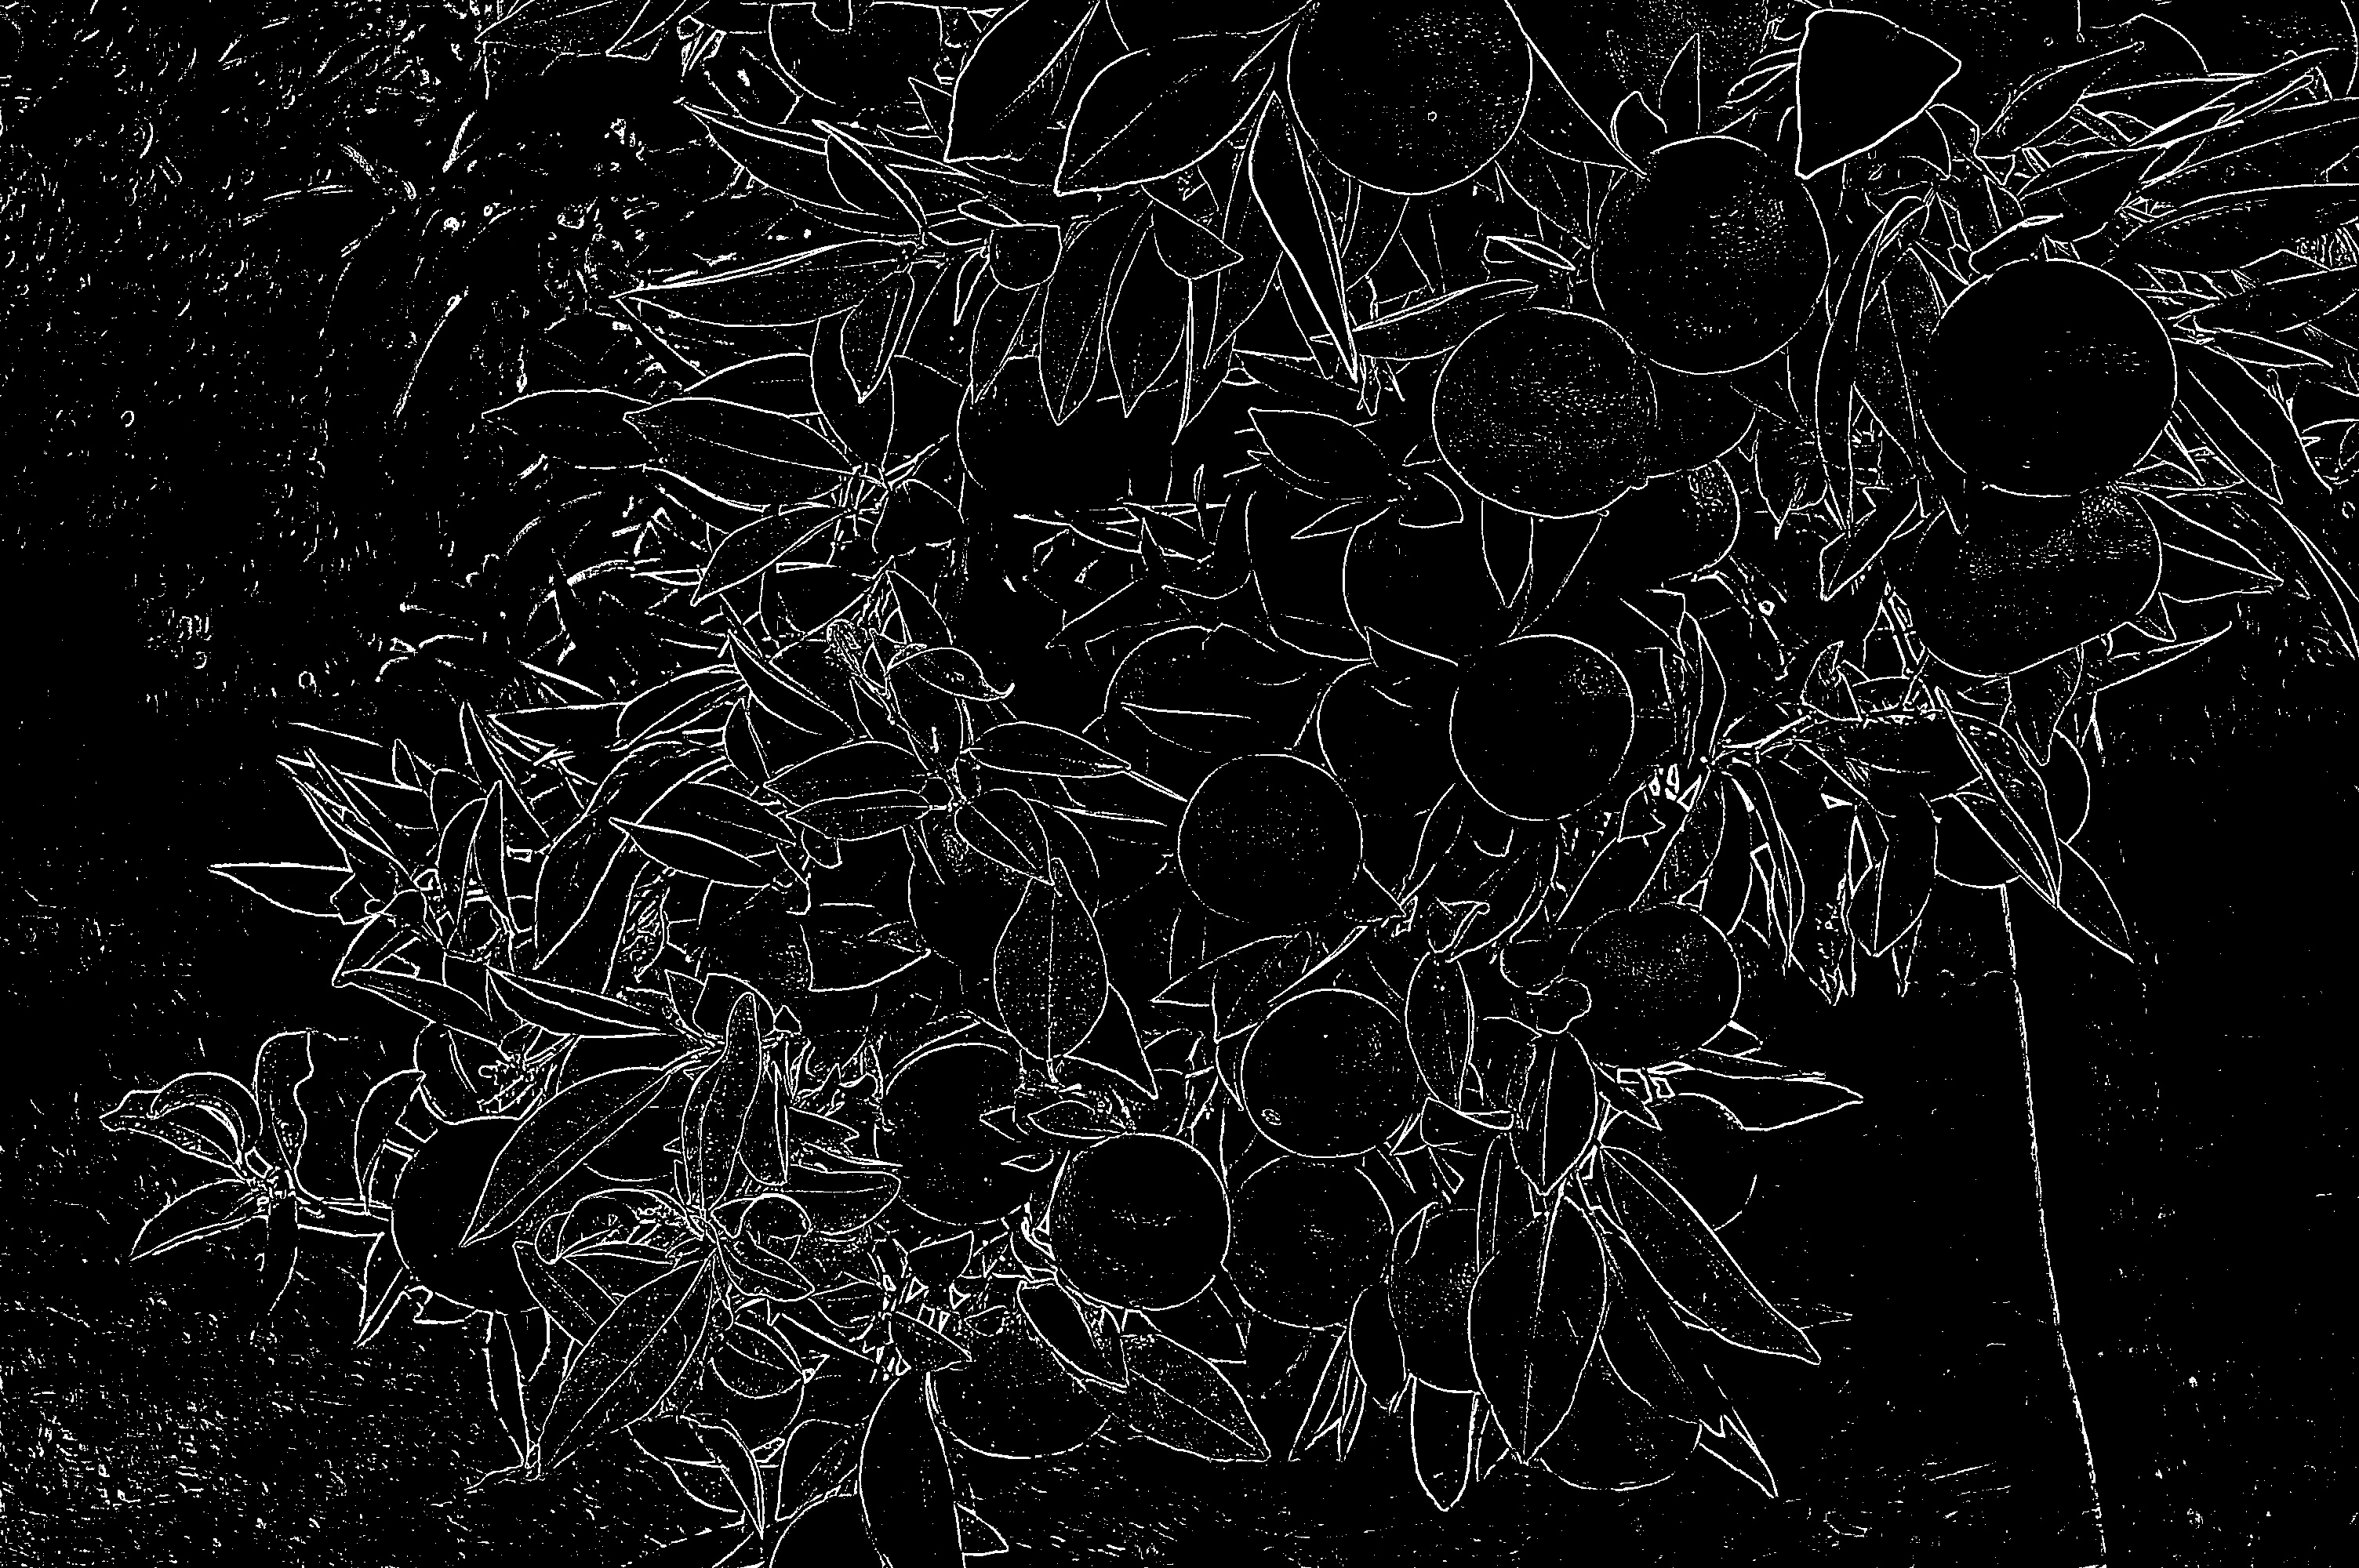
\includegraphics[width=\linewidth]{citrus1/citrus1_mean.jpg}
  	\caption{Result of step 2}
  \end{subfigure}\par\medskip
  
  \begin{subfigure}{.3\linewidth}
  	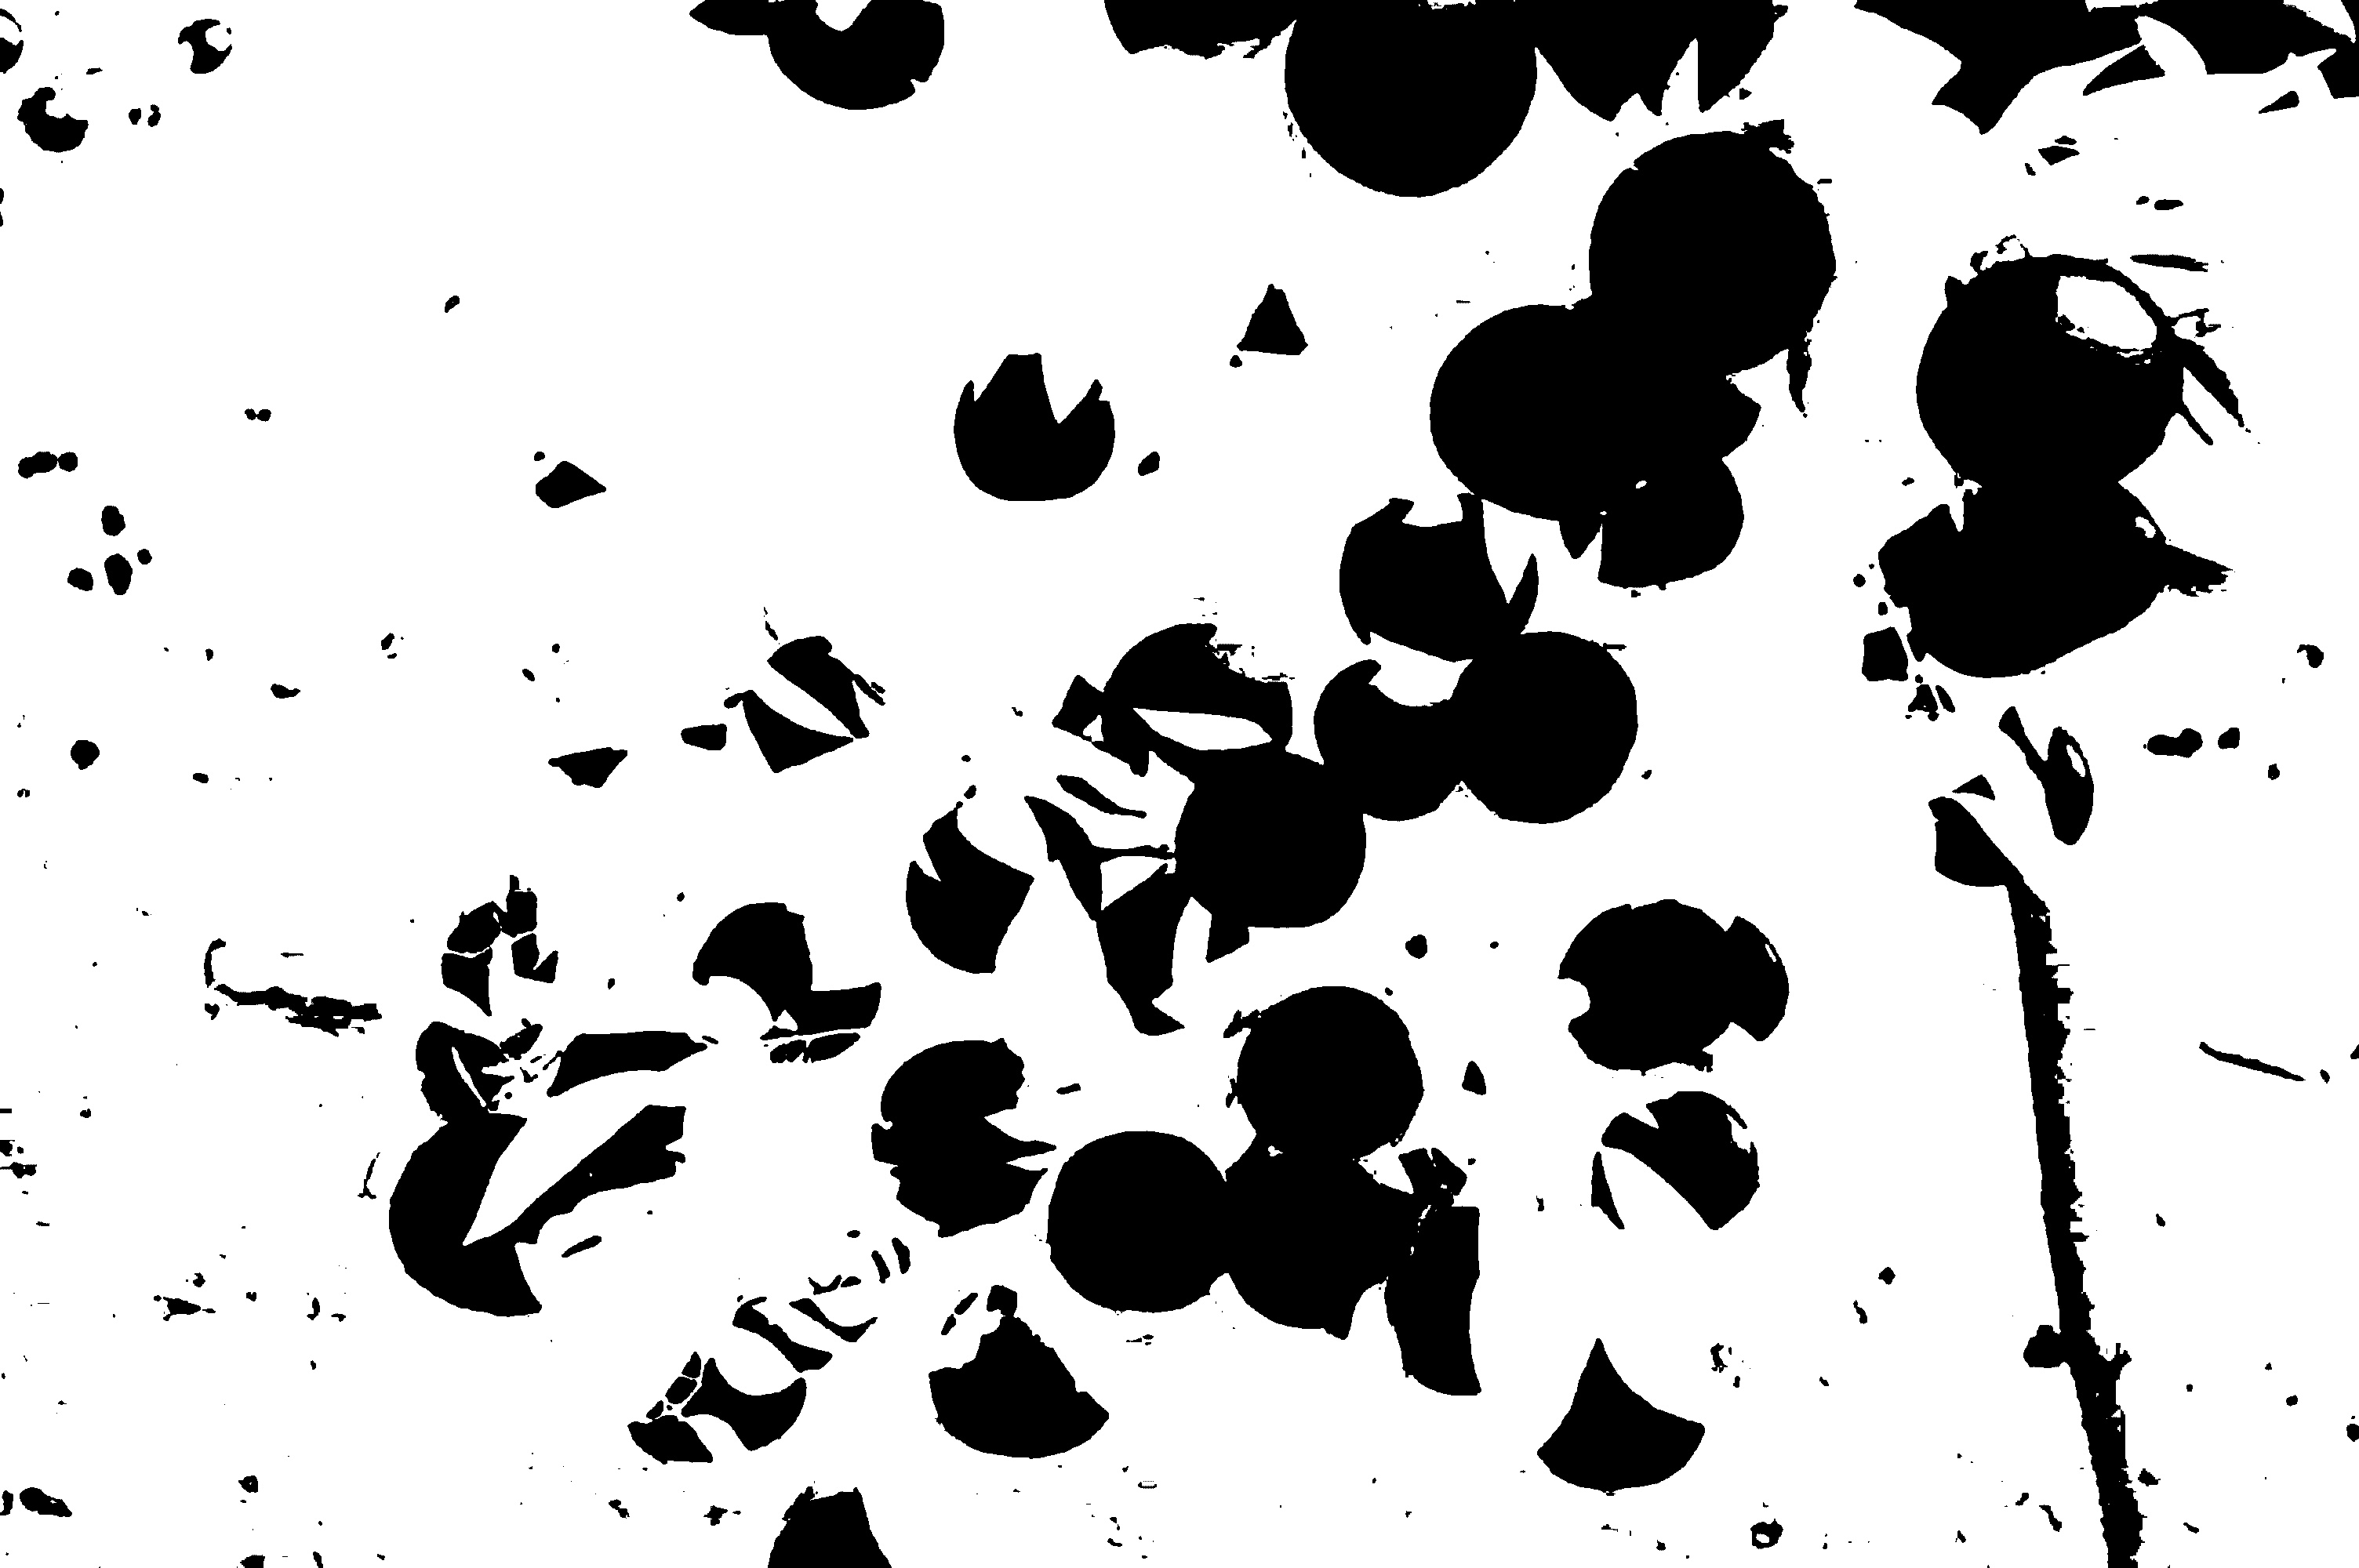
\includegraphics[width=\linewidth]{citrus1/citrus1_cr.jpg}\hfill
     	\caption{Result of step 3}
  \end{subfigure}
  \begin{subfigure}{.3\linewidth}
  	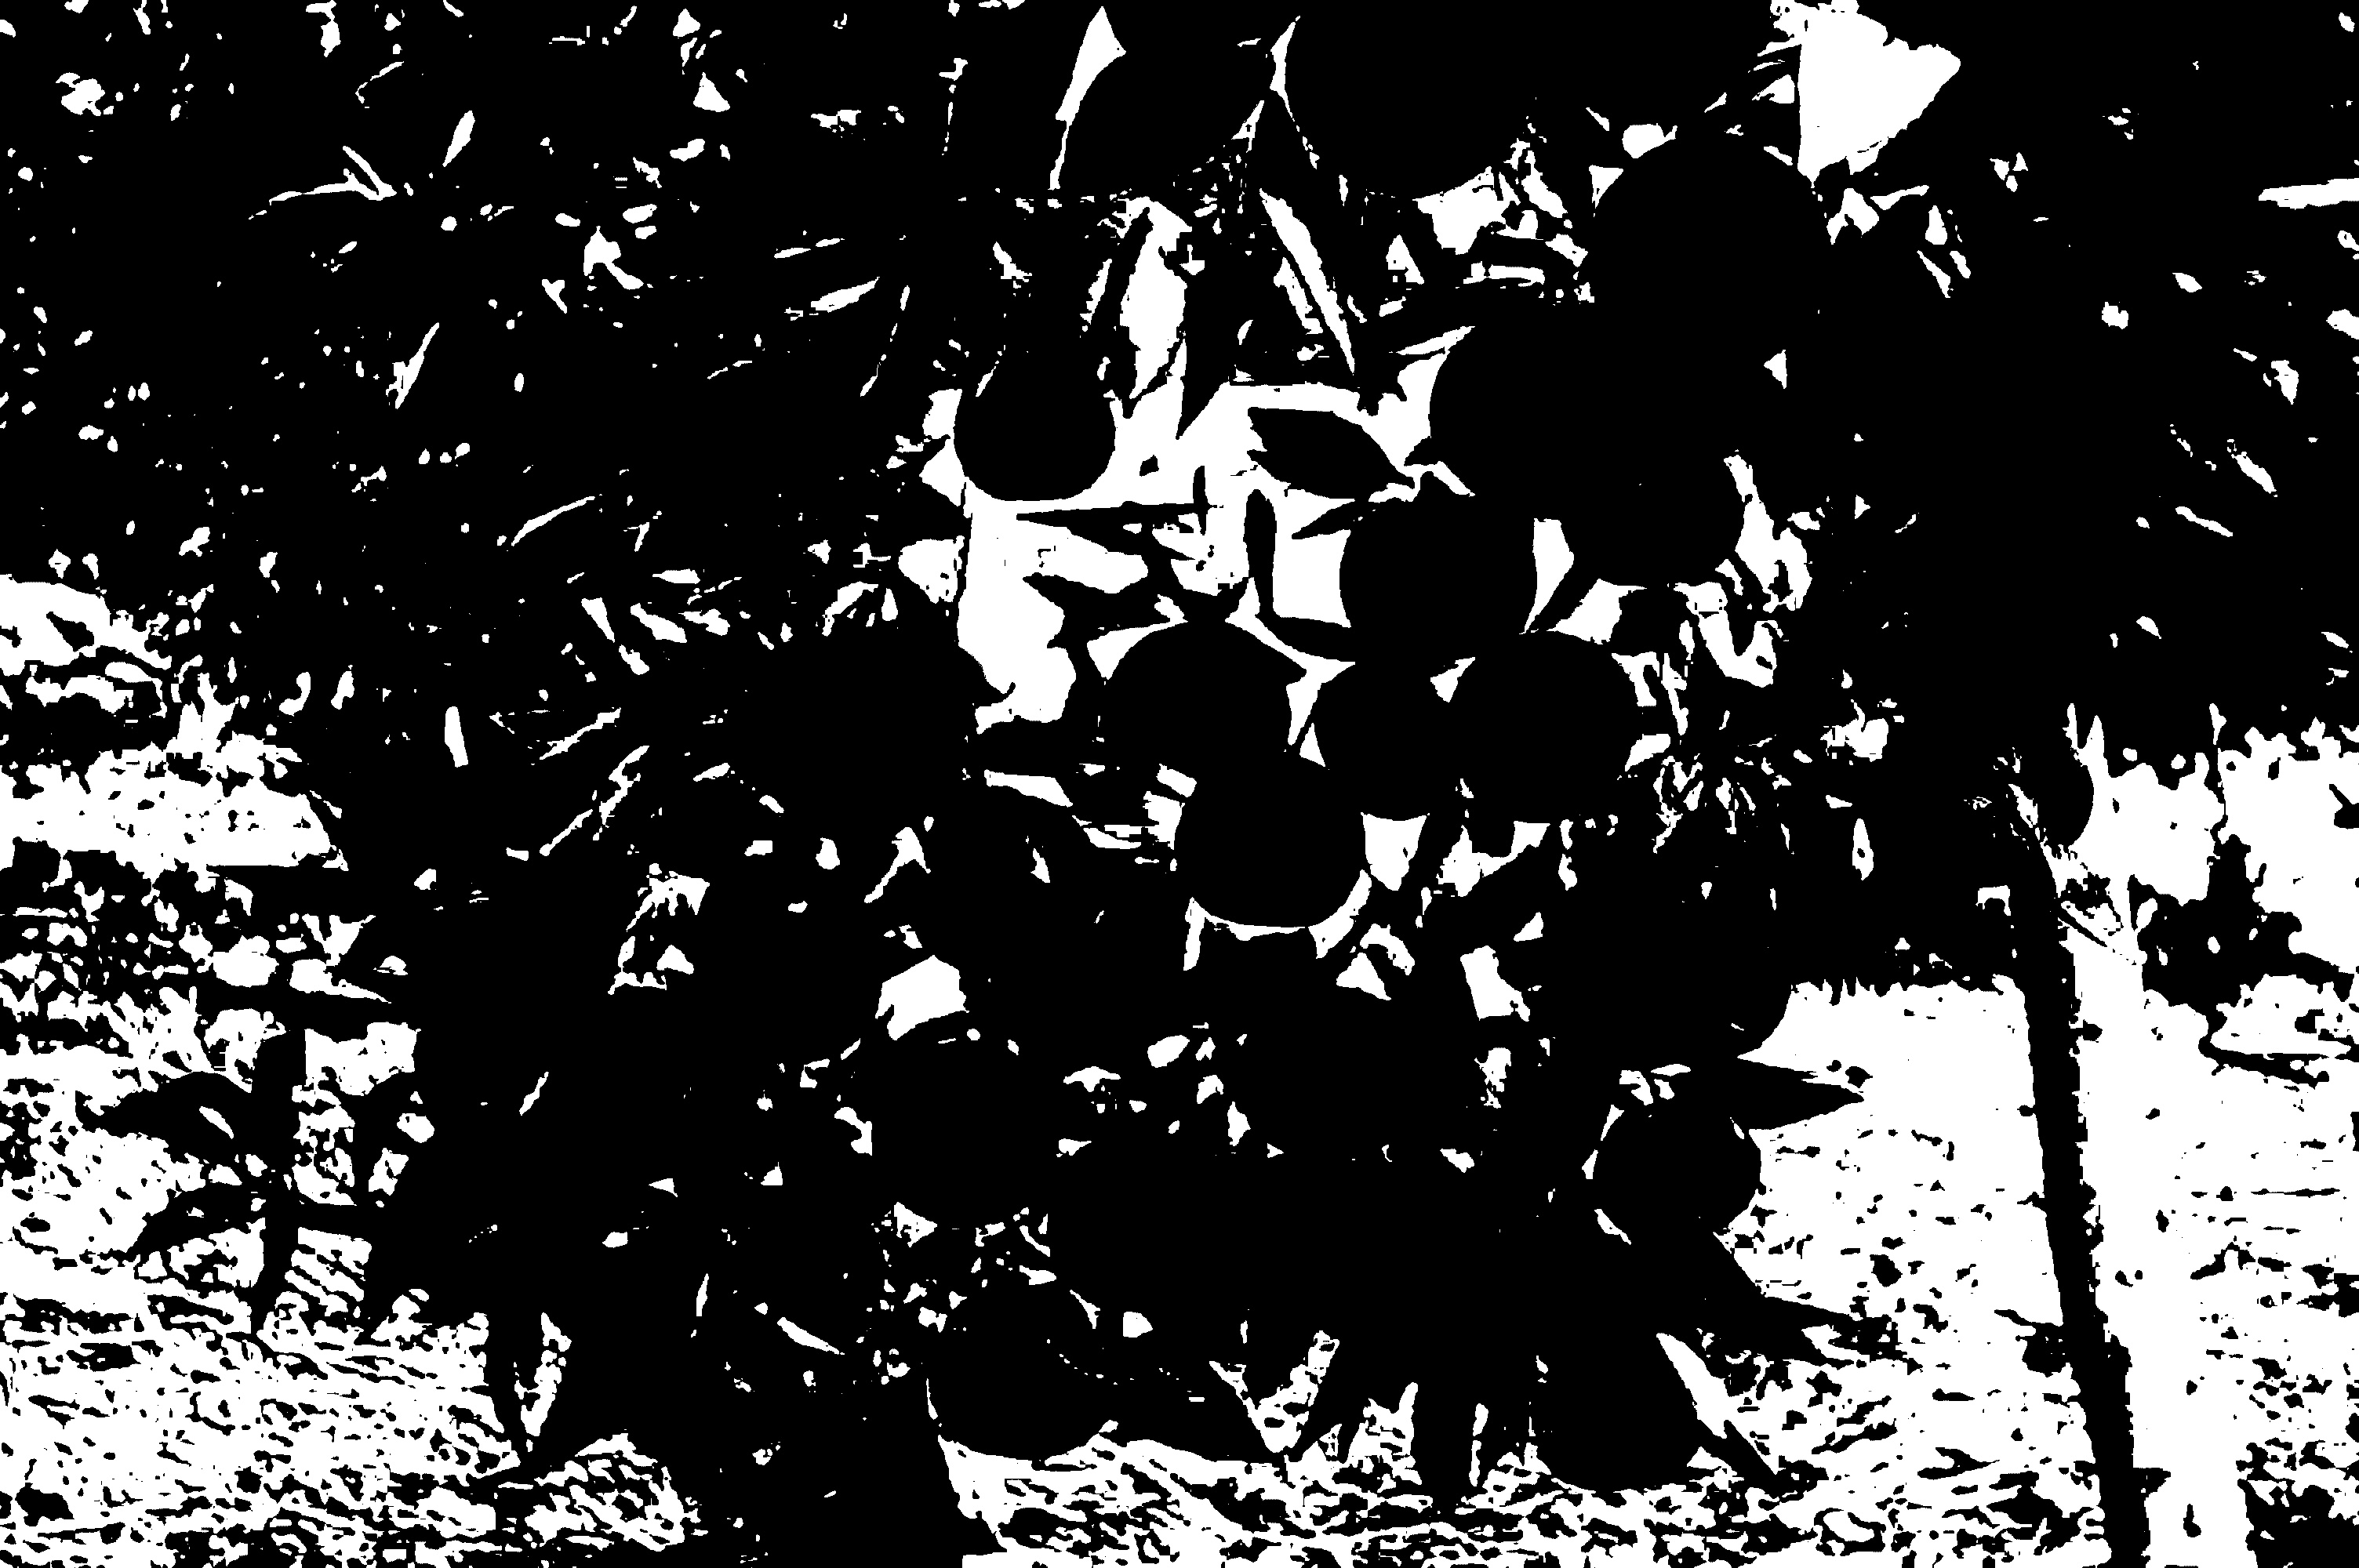
\includegraphics[width=\linewidth]{citrus1/citrus1_cb.jpg}\hfill
     	\caption{Result of step 4}
  \end{subfigure}
  \begin{subfigure}{.3\linewidth}
  	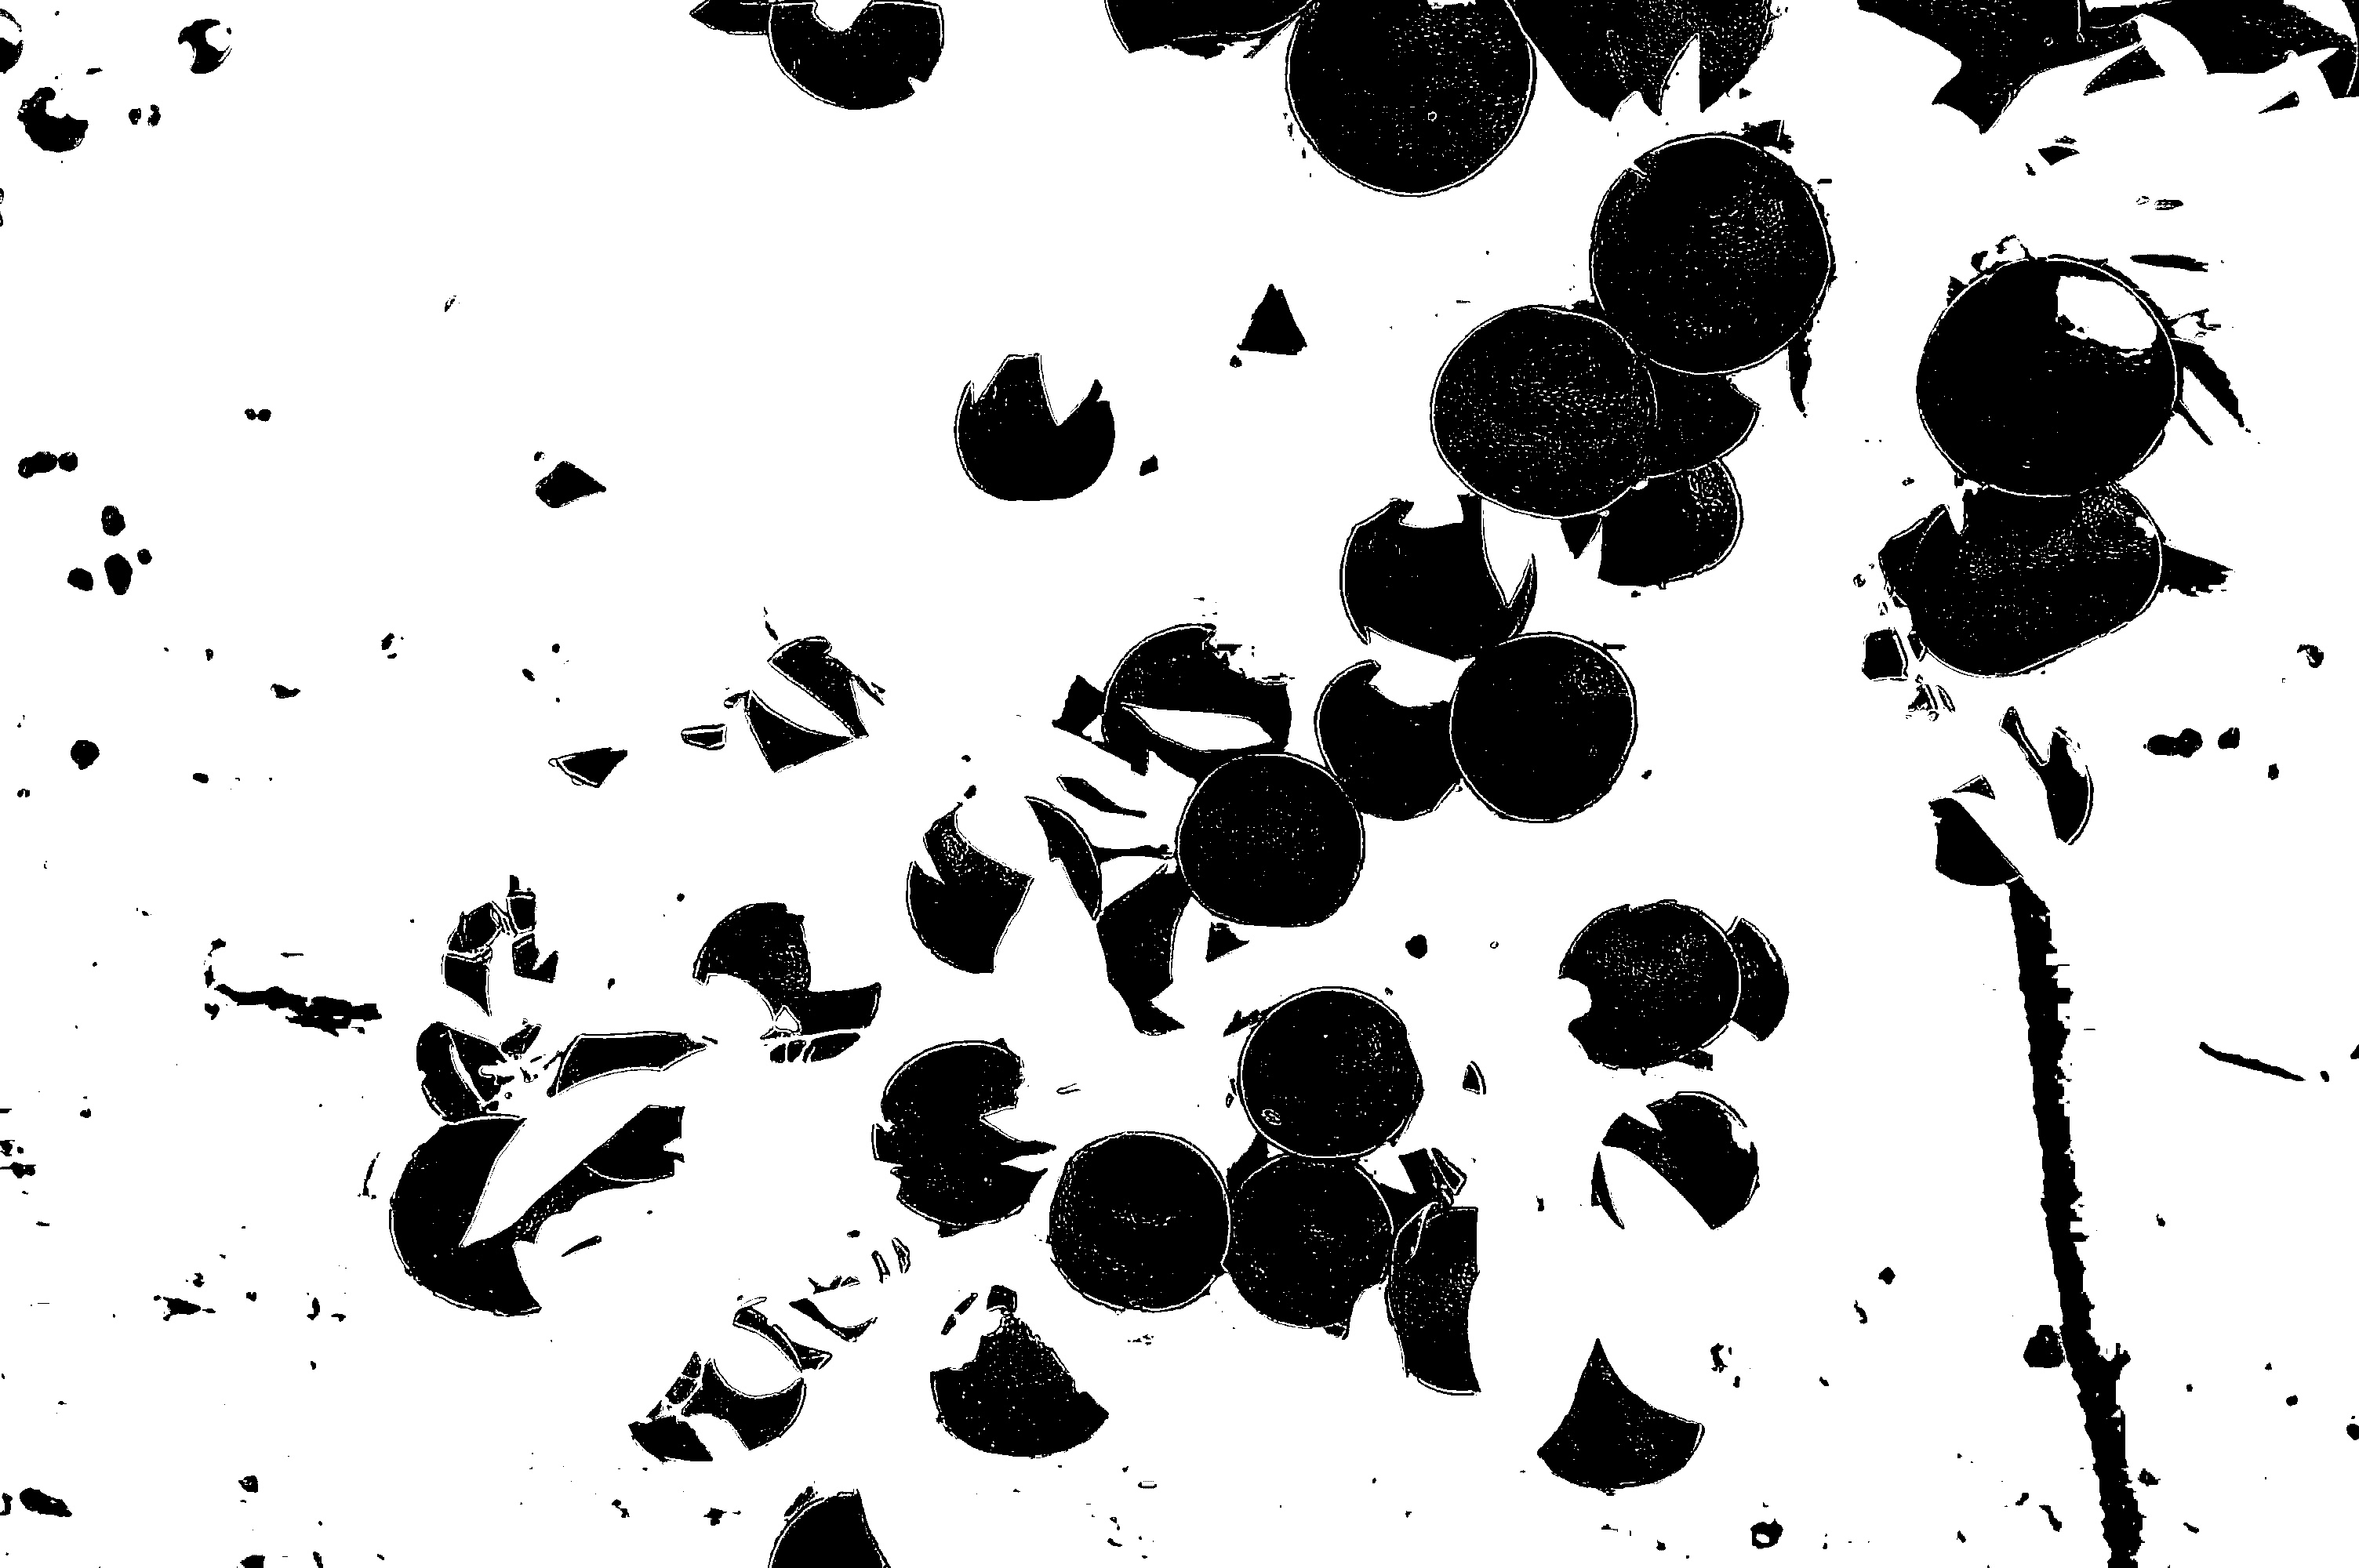
\includegraphics[width=\linewidth]{citrus1/citrus1_mask.jpg}
  	\caption{Result of step 5}
  \end{subfigure}\par\medskip
  \begin{subfigure}{.49\linewidth}
  	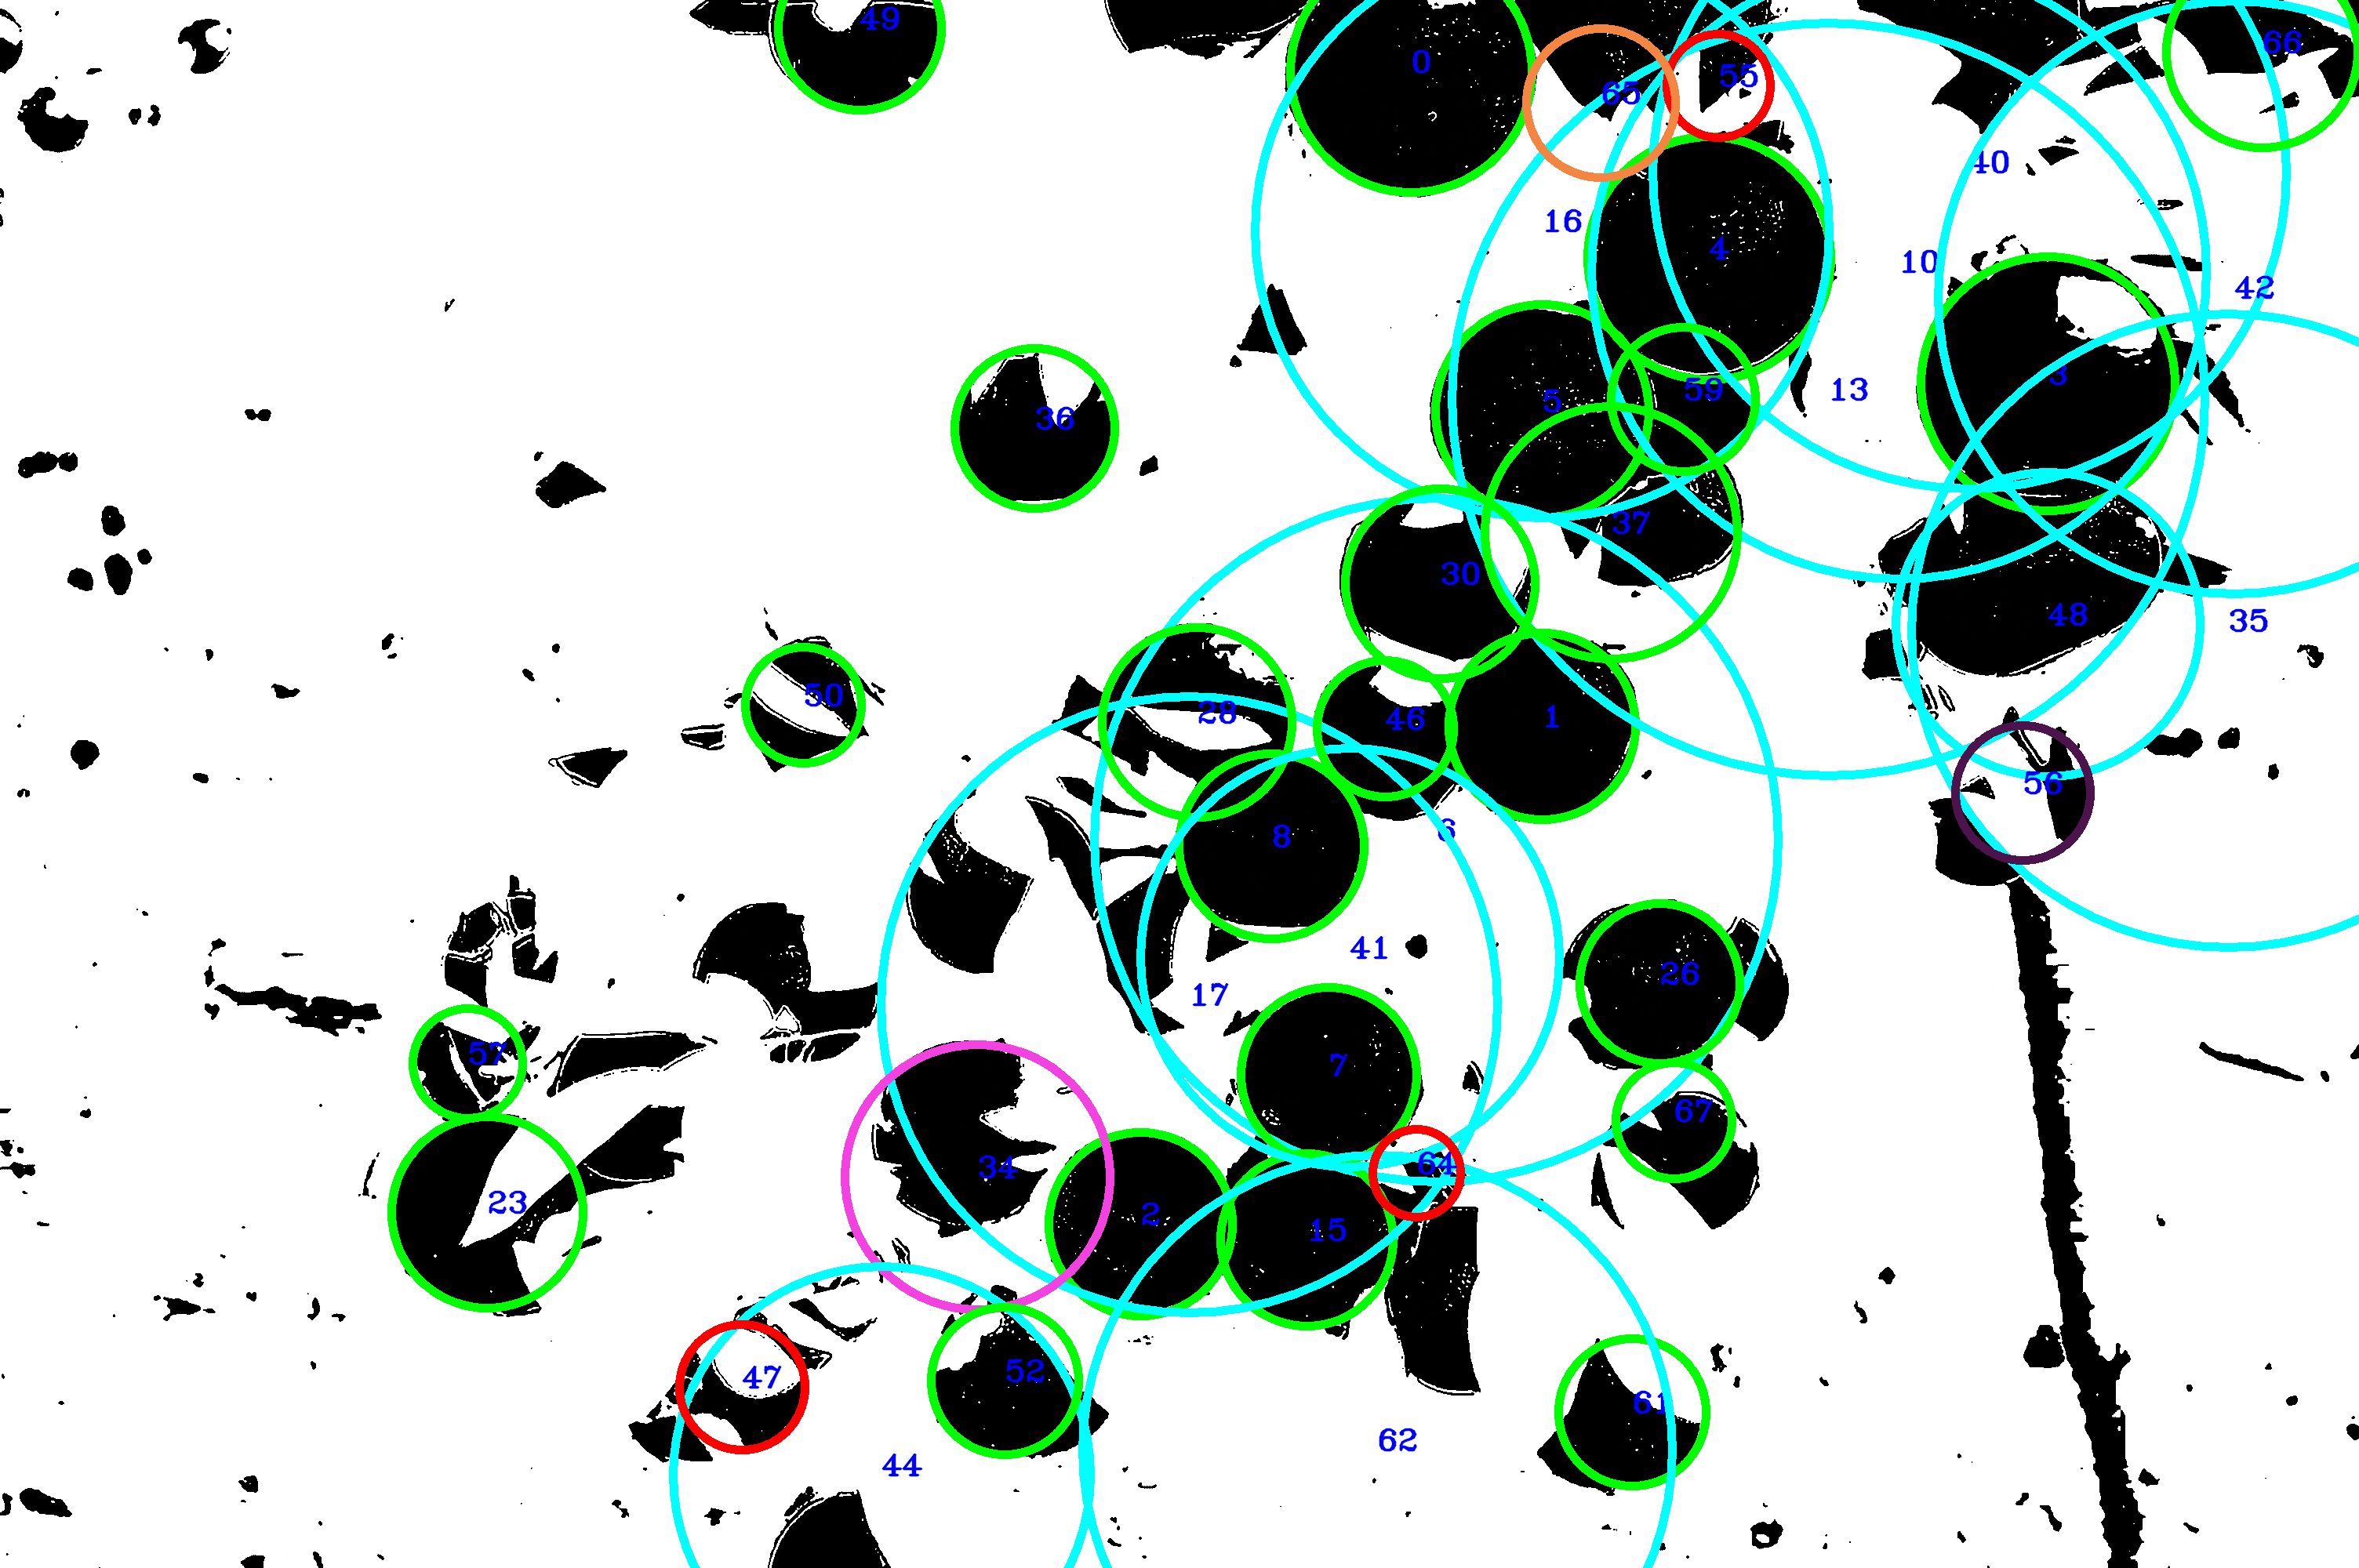
\includegraphics[width=\linewidth]{citrus1/citrus1_circles_mask.png}\hfill
	   	\caption{Result of step 6a}
  \end{subfigure}
  \begin{subfigure}{.49\linewidth}
  	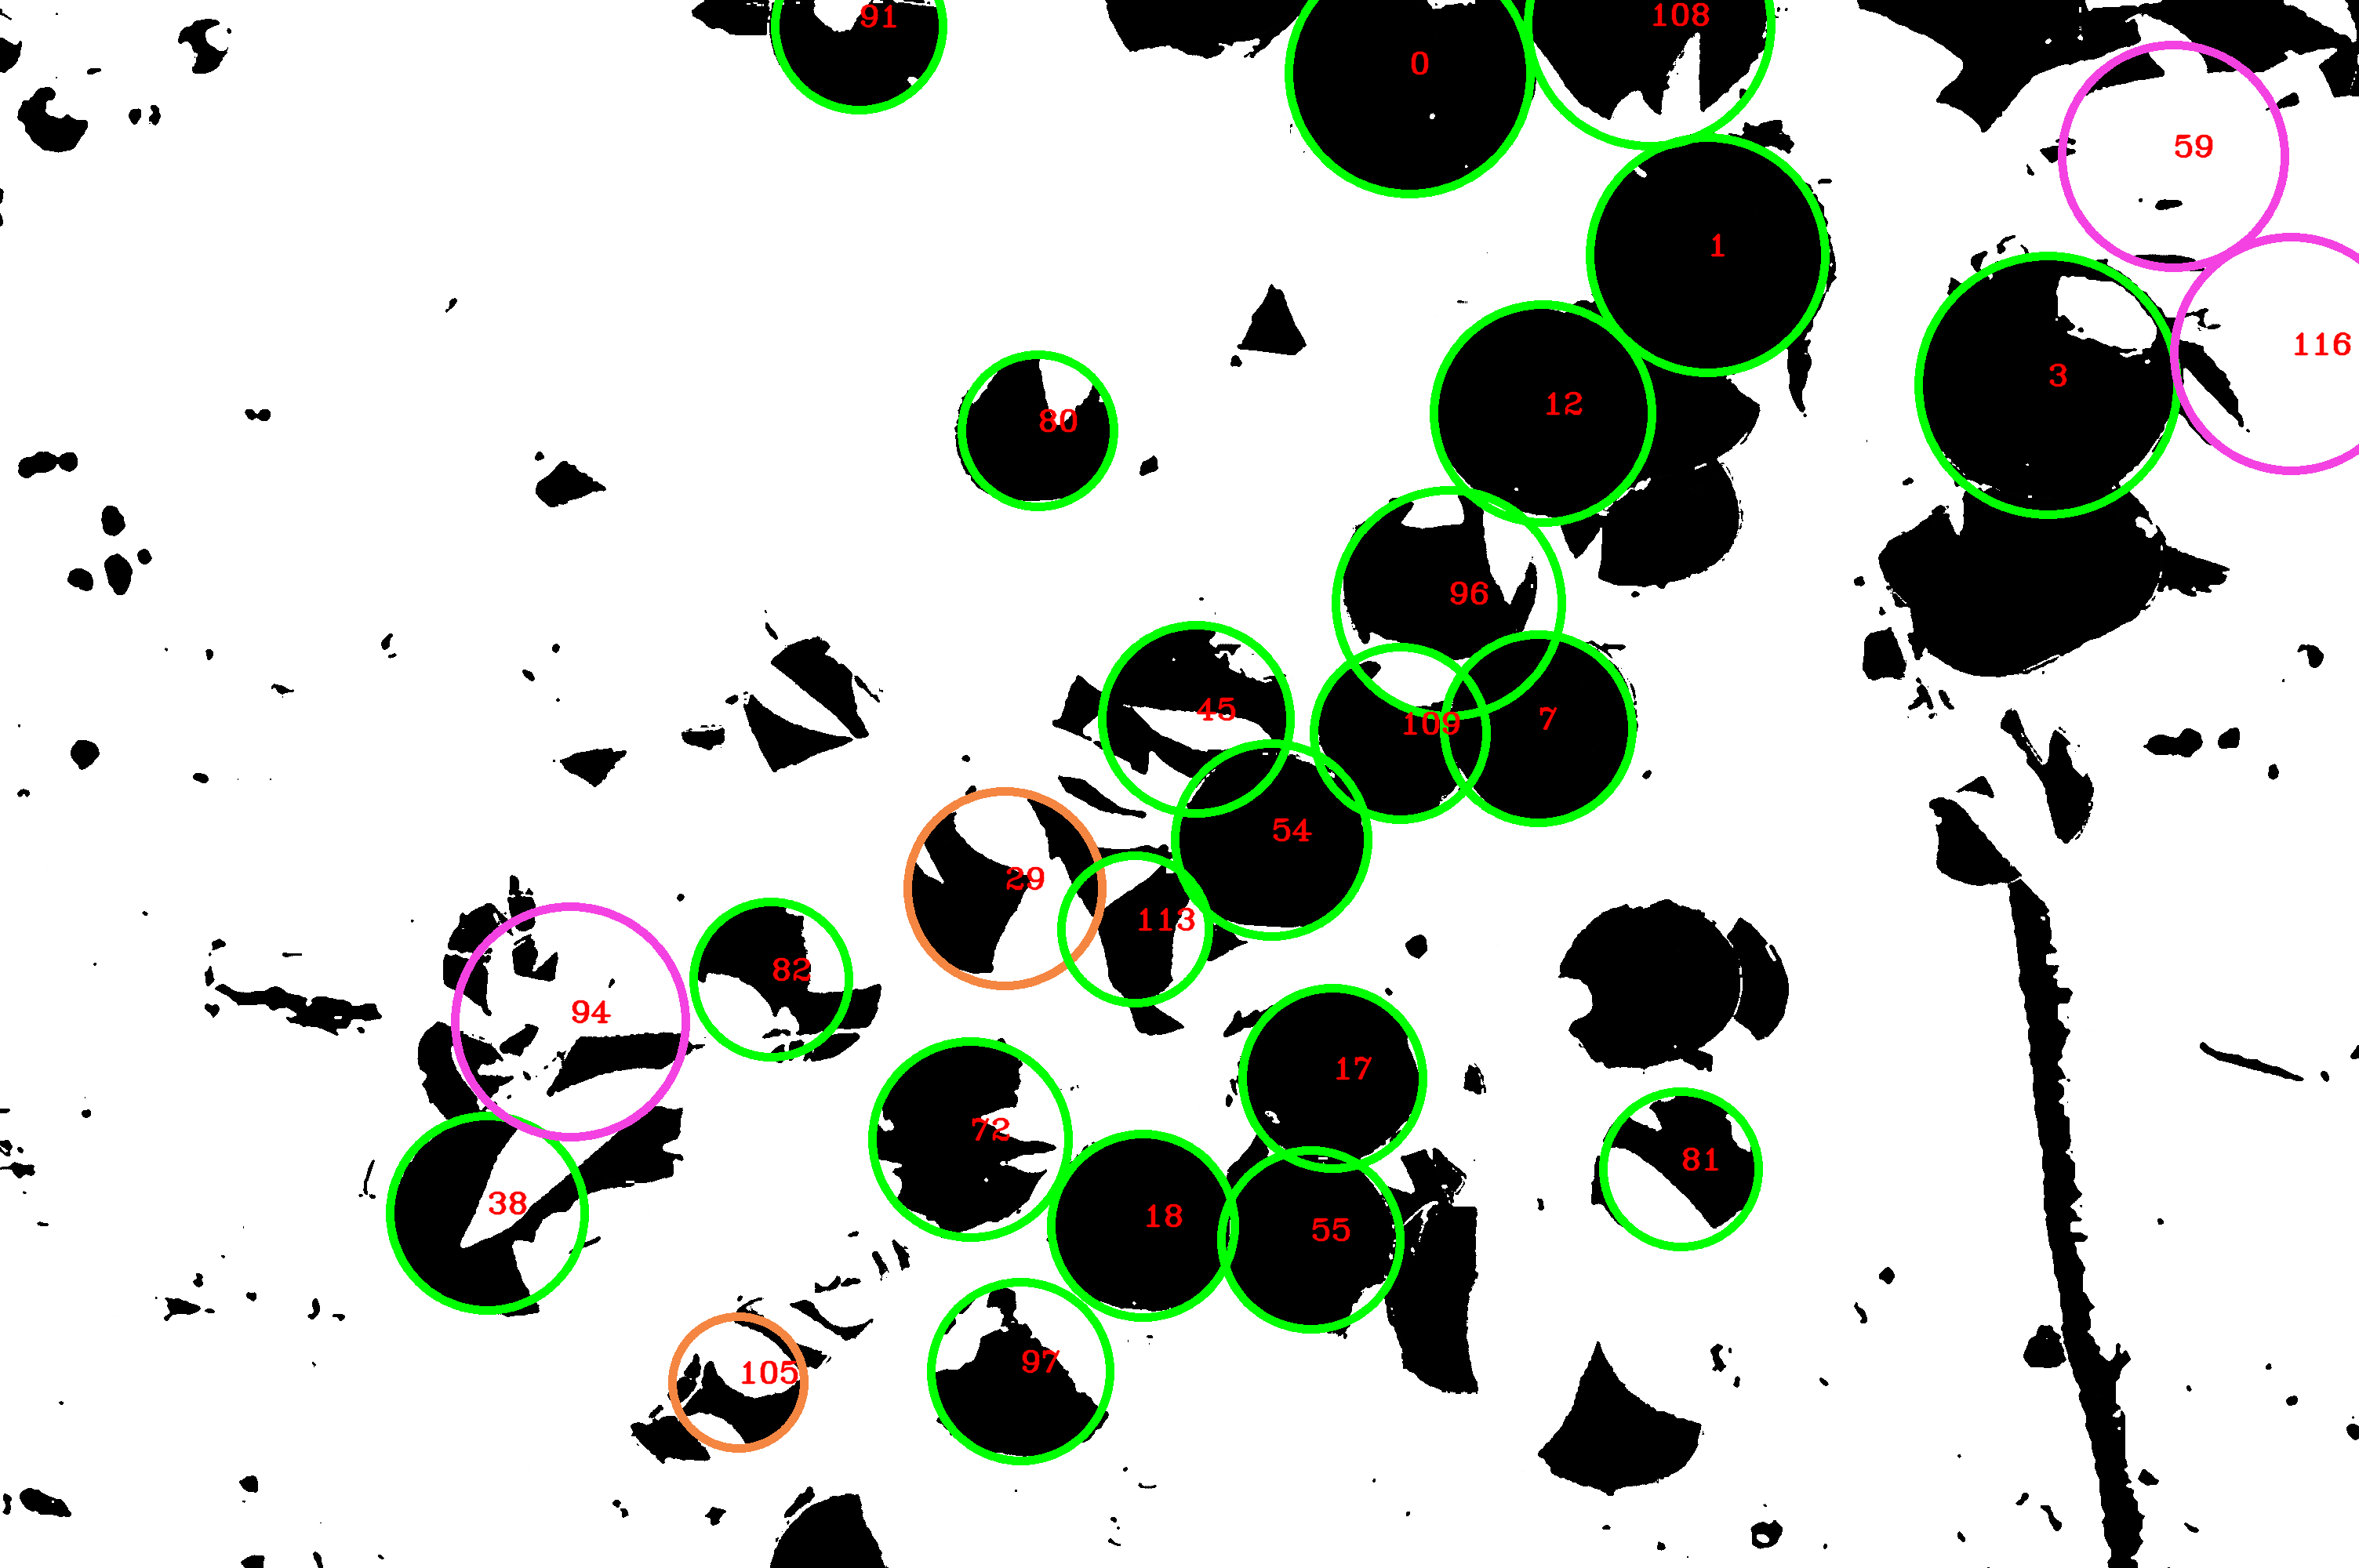
\includegraphics[width=\linewidth]{citrus1/citrus1_circles.png}\hfill
 	 \caption{Result of step 6b}
  \end{subfigure}
  \caption{An example image going through each step to detect the oranges within the image} \
\end{figure}


\section{Discussion}

\subsection{Limitations} \label{sec:limitations}

When we were testing our algorithm we noticed that it worked significantly better on images larger than 1300x1300px. It also does not work on images where the diameter of the oranges is greater than half of the screen size, or if the oranges are very small (less then 150px) This is a direct result of the value that was chosen for the minimum distance between circles in algorithm \ref{circleCountAlg}. We determined that this short coming can be easily overcome by using image resolutions above that size. In the application where this algorithm would be used the image quality would be known and the zoom of the image would be consistent allowing the mentioned shortcomings to be overcame. 



\section{Psudo code}

\subsection{Circle Filtering}


\begin{algorithm} 
    \SetKwInOut{Input}{Input}
    \SetKwInOut{Output}{Output}

    \underline{function CheckOverlap} $(foundMask, circle, img, whitePixels)$\;
    \Input{mask where the taken regions are set to 1 and untaken set to  0 $foundMask$}
    \Input{the circle that is being checked $circle$}
    \Input{the binarized image of oranges $img$}
    \Input{percentage of pixels that are white $whitePixels$}
    \Output{$if the circle should be ignored$}
    
    \uIf{$whitePixels \leq 50$}
    {
    	return True
    }
        
    circleMask = fillMask(img.size, circle)
    
    areaNotTaken = 0
    
    areaNewOrangeInFrame = 0
    
    areaFilledNotTaken = 0
    
    \For{$i \in img.height$}
    {
    	 \For{$j \in img.width$}
	 {
	 	\lIf{$\neg foundMask[i,j] \land circleMask$}
		{
			areaNotTaken++
		}
		
		\lIf{$circleMask$}
		{
			areaNewOrangeInFrame++
		}
		
		\lIf{$\neg foundMask[i,j] \land circleMask \land img[i,j]$}
		{
			areaFilledNotTaken++
		}
	 }
    }
    
    /* check that orange is distinct */
    
    \lIf{$areaNotTaken / areaNewOrangeInFrame  \cdot 100 < 10$}
     {
	return False
    }
    
    /* check that non overlaping section is partly filled */
    
    \lIf{$areaFilledNotTaken / areaNewOrangeInFrame  \cdot 100 < 10$}
     {
	return False
    }
    
    return True
    
    \caption{Determine if too much of the circle is already taken by another circle} \label{CheckOverlapAlg}
\end{algorithm}



\begin{algorithm} 
    \SetKwInOut{Input}{Input}
    \SetKwInOut{Output}{Output}

    \underline{function OrangeCount} $(circle, img,)$\;
    \Input{the circle that is being checked $circle$}
    \Input{the binarized image of oranges $img$}
    \Output{percentage of pixels that are white $whitePixels$}
    
        
    circleMask = fillMask(img.size, circle)
    
    circleArea = $  \cdot \pi \cdot circle.radius^2$
    
    numOutOfFrame = circleArea
   
    numOrange = 0
    
    
    \For{$i \in img.height$}
    {
    	 \For{$j \in img.width$}
	 {
	 	numOutOfFrame--
		
	 	\lIf{$img[i,j] \land circleMask$}
		{
			numOrange++
		}
	 }
    }
    
    /* check that enough is in frame*/
    
    \lIf{$numOutOfFrame / circleArea  \cdot 100 > 40$}
     {
	numOrange += numOutOfFrame
    }
    
    percentFilledInFrame = numOrange / numTotal * 100
    
    percentFilled = numOrange / (numTotal - numOutOfFrame) * 100
    
    return min(percentFilledInFrame, percentFilled)
    
    
    \caption{Count the number of pixels that are within the circle that have been marked as orange} \label{OrangeCountAlg}
\end{algorithm}



\bibliographystyle{ieeetr}
\bibliography{reference}





\vspace{12pt}

\end{document}
